\documentclass[times, utf8, zavrsni, numeric]{fer}
\usepackage{booktabs}
\usepackage{caption}
\usepackage{subcaption}
\usepackage{algorithm}
\usepackage{algpseudocode}
\usepackage{pdfpages}
\graphicspath{ {./resursi/slike} }
\begin{document}

% TODO: Navedite broj rada.
\thesisnumber{848}

% TODO: Navedite naslov rada.
\title{Igranje igre \textit{2048} korištenjem Kartezijevog genetskog programiranja}

% TODO: Navedite vaše ime i prezime.
\author{Paulo Erak}

\maketitle

% Ispis stranice s napomenom o umetanju izvornika rada. Uklonite naredbu \izvornik ako želite izbaciti tu stranicu.
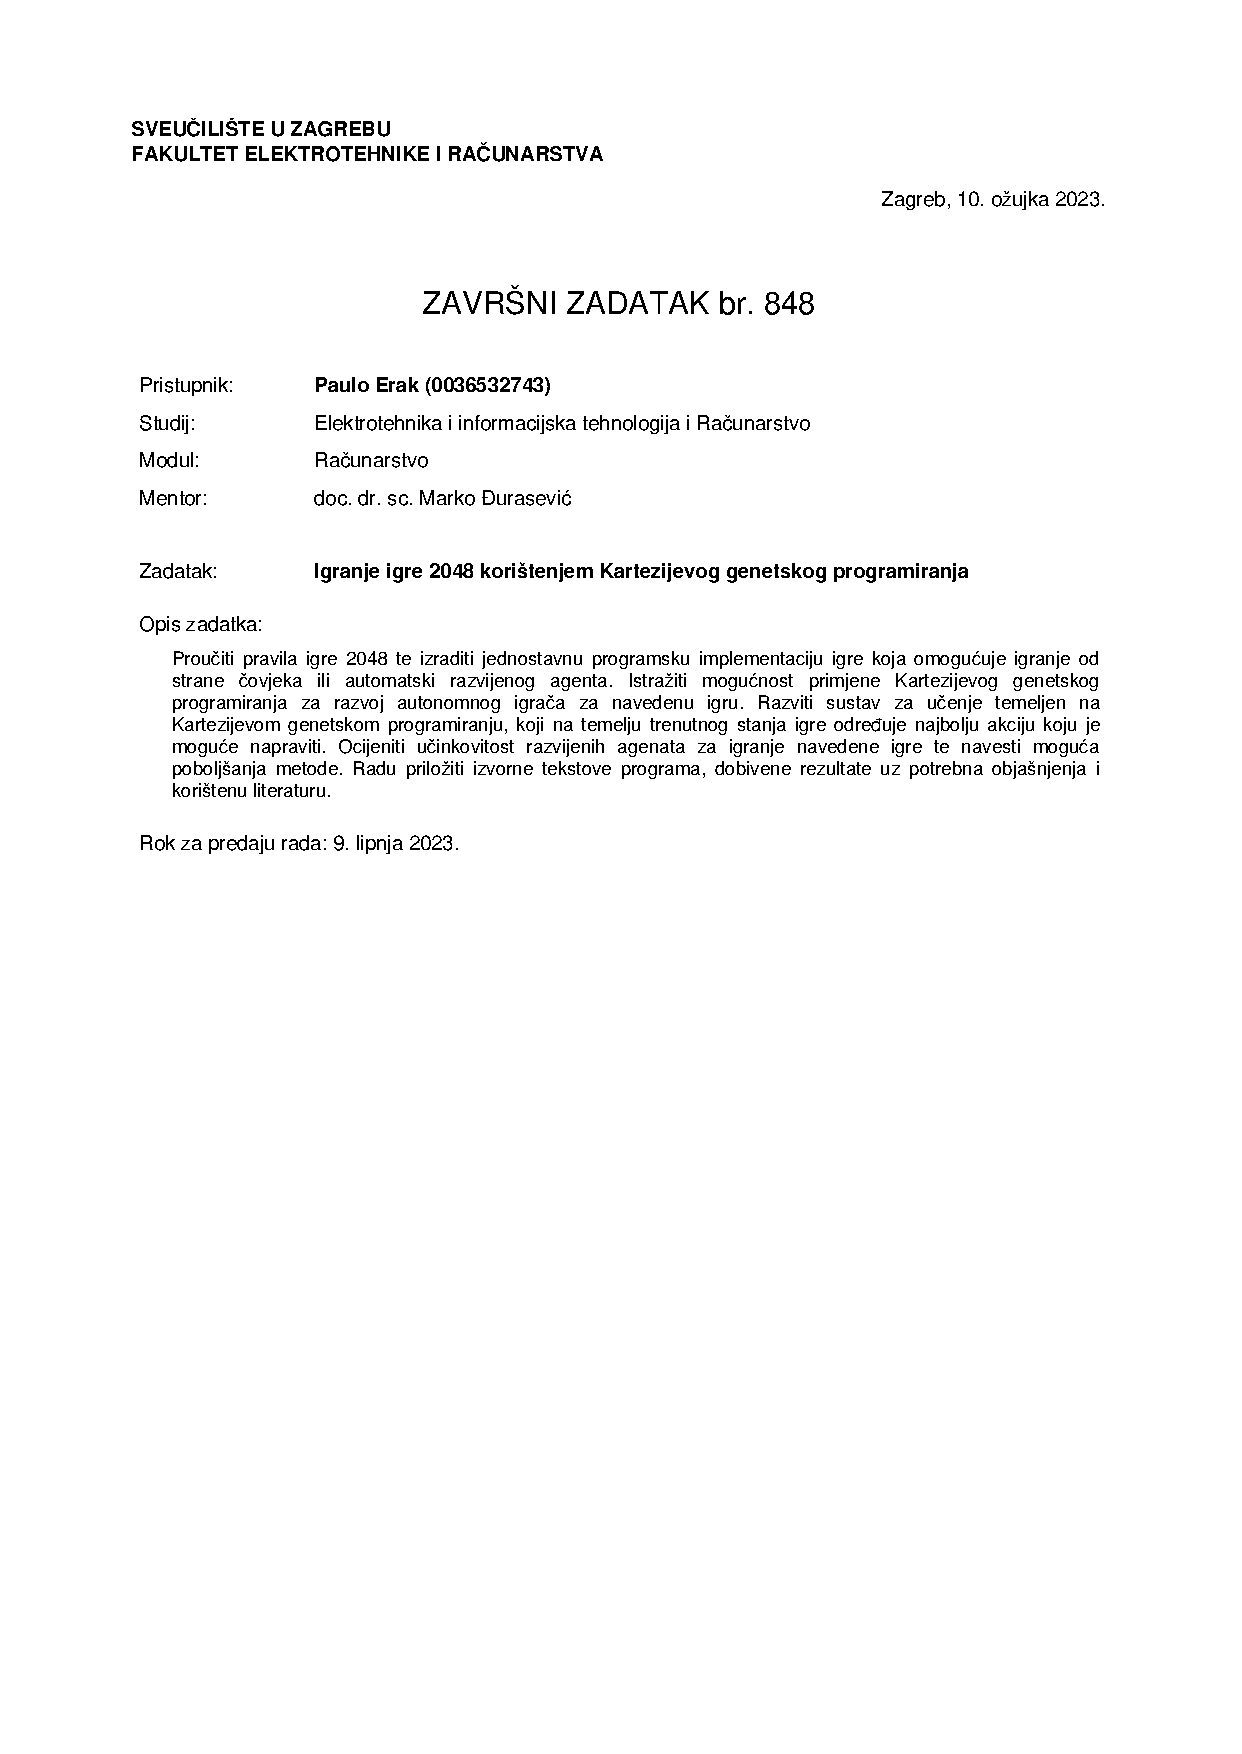
\includepdf[pages=-]{hr_0036532743_73.pdf}

% Dodavanje zahvale ili prazne stranice. Ako ne želite dodati zahvalu, naredbu ostavite radi prazne stranice.
\zahvala{\par Zahvaljujem se mentoru doc. dr. sc. Marku Đuraseviću što je vrlo ugodnom radnom atmosferom, savjetima, preporukama literature i strpljenjem uvelike olakšao izradu ovog završnog rada.\par
	Zahvaljujem se majci, ocu, bratu Jakovu i svoj svojoj obitelji na konstantnoj potpori i bodrenju u svemu što sam radio. \par
	Zahvaljujem se svim svojim prijateljima koji su bili uz mene i koji su mi bili velika potpora kroz cijeli preddiplomski studij, a i prije njega.\par
	Bez ovih ljudi ne bih bio tu gdje jesam i tko jesam. Uistinu veliko hvala.\newline
	
	}

\tableofcontents

\chapter{Uvod}
Iako je većina igara napravljena za dvoje ili više igrača, razvojem tehnologije, a posebno računala, počinju se razvijati igre za samo jednog igrača. U njima je najčešći cilj dobiti najbolji/najveći rezultat koristeći pravila po kojima igra funkcionira na optimalan način. Tako se često igri pristupa kao slagalici koju u što manje poteza pokušavamo složiti što bolje, a svaki od naših poteza se boduje i utječe na sljedeće poteze.\par
Igra \textit{2048} upravo je takva igra napravljena za jednog igrača. Cilj igre je dobiti što veći rezultat koji je sam po sebi zbroj novostvorenih brojeva na ploči ispred nas. Imamo vrlo jednostavne poteze: pomicanje svih dijelova ploče lijevo, desno, gore ili dolje. Prilikom pomicanja, elementi koji su isti i susjedni, a nalaze se jedan drugome na putanji, spajaju se i time otvaraju prostor na ploči. Nakon svakog poteza se na nasumično otvoreno mjesto stavlja novi element. Igra se čini poprilično jednostavna za shvatiti te ćemo u kasnijem poglavlju vidjeti još neke pojedinosti igre.\par
Unatoč svojoj jednostavnosti, igra može postati podosta kompleksna. Upravljanje praznim prostorom te općenita prostorna organizacija elemenata postaje zahtjevnija kako vrijeme prolazi. Igrač će se prije ili kasnije naći u situaciji kad mu je ploča ispunjena do kraja i više nije u stanju napraviti ijedan potez. U tom trenutku igra se završava.\par 
Cilj ovog rada je stvoriti agenta ili populaciju agenata koristeći Kartezijevo genetsko programiranje koji bi na osnovu stanja ploče napravili što bolji potez u kontekstu cijele partije.\par
U sklopu ovog rada bavit ćemo se konceptima genetskog programiranja, Kartezijevog genetskog programiranja, razvojem agenata kroz generacije, implementacijom specifičnom za ovaj rad, njezinim rezultatima i diskusijom o rezultatima.


\chapter{Igra 2048}
\quad U ovom poglavlju ulazimo dublje u pravila i funkcioniranje igre. Fokus će biti stavljen na neke pojedinosti koje su uzete u obzir prilikom implementacije ovog rada.\par 
Odmah se stavlja naglasak na to kako ovaj rad nije napravljen nad originalnom verzijom igre \textit{2048} već nad verzijom koju su razvili Krešo Orešković i Paulo Erak u sklopu projekta na Fakultetu elektrotehnike i računarstva (FER) pod mentorom Markom Đurasevićem. \par
U samom uvodu pokrili smo neke od najvažnijih elemenata i pravila igre koja su sadržana u obje verzije: \textit{Cilj igre je dobiti što veći rezultat koji je sam po sebi zbroj novostvorenih brojeva na ploči ispred nas. Imamo vrlo jednostavne poteze: pomicanje svih dijelova ploče lijevo, desno, gore ili dolje. Prilikom pomicanja, elementi koji su isti i susjedni, a nalaze se jedan drugome na putanji, spajaju se i time otvaraju prostor na ploči. Nakon svakog poteza se na nasumično otvoreno mjesto stavlja novi element.}\par
 Uzevši to u obzir, verzije igre nisu iste i neka pravila se razlikuju. Ta pravila bit će posebno naglašena u potpoglavlju \textit{Verzija igre korištena u radu}.\par 


\section{Originalna igra \textit{2048}}
Originalnu igru \textit{2048} napravio je talijanski programer, Gabriele Cirulli, koji je svoj rad \cite{2048og} postavio na internetsku uslugu za pohranu i upravljanje verzijama koda, GitHub.\par 
Igra se sastoji od nekoliko grafičkih elemenata: ploča (najčešća dimenzija je 4x4), kvadrati raznih boja koji sadrže brojeve (potencije broja 2) te se nalaze na ploči, brojači koji prikazuju trenutni i  najbolji rezultat i gumb za ponovo pokretanje igre.\newline
	\begin{figure}[h]
		\begin{subfigure}{0.5\textwidth}
			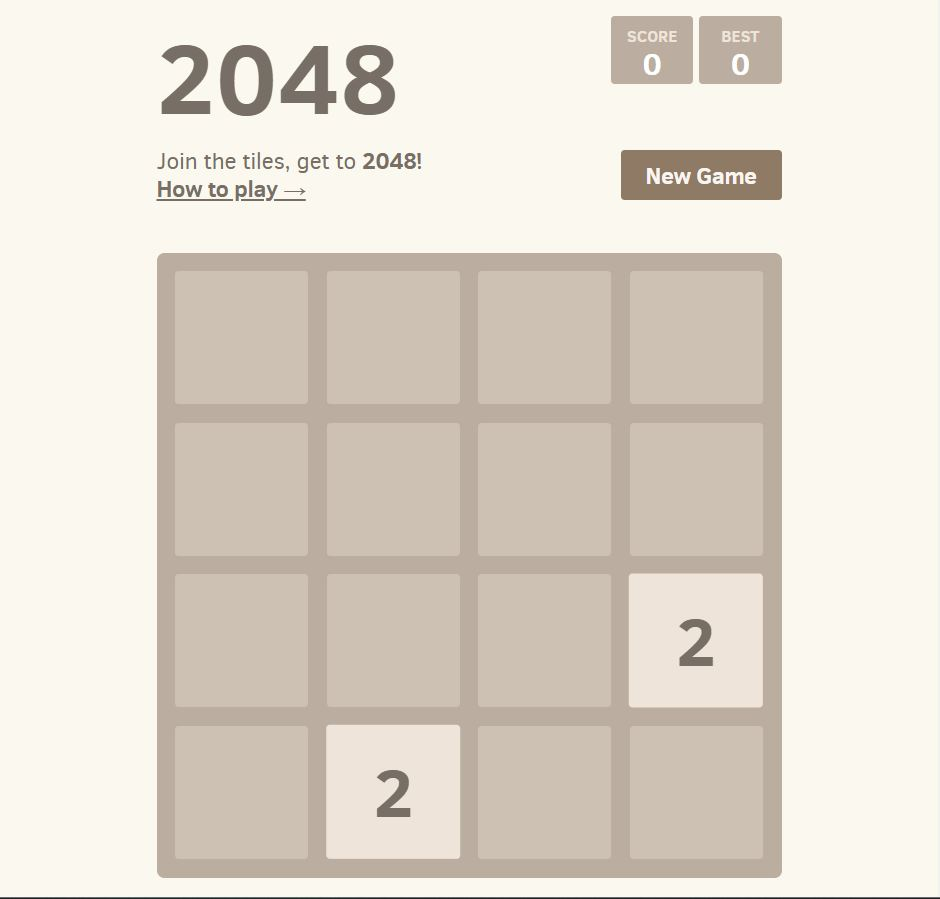
\includegraphics[width=0.9\linewidth, height=6cm]{originalni_2048} 
			\caption{Početno stanje}
		\end{subfigure}
		\begin{subfigure}{0.5\textwidth}
			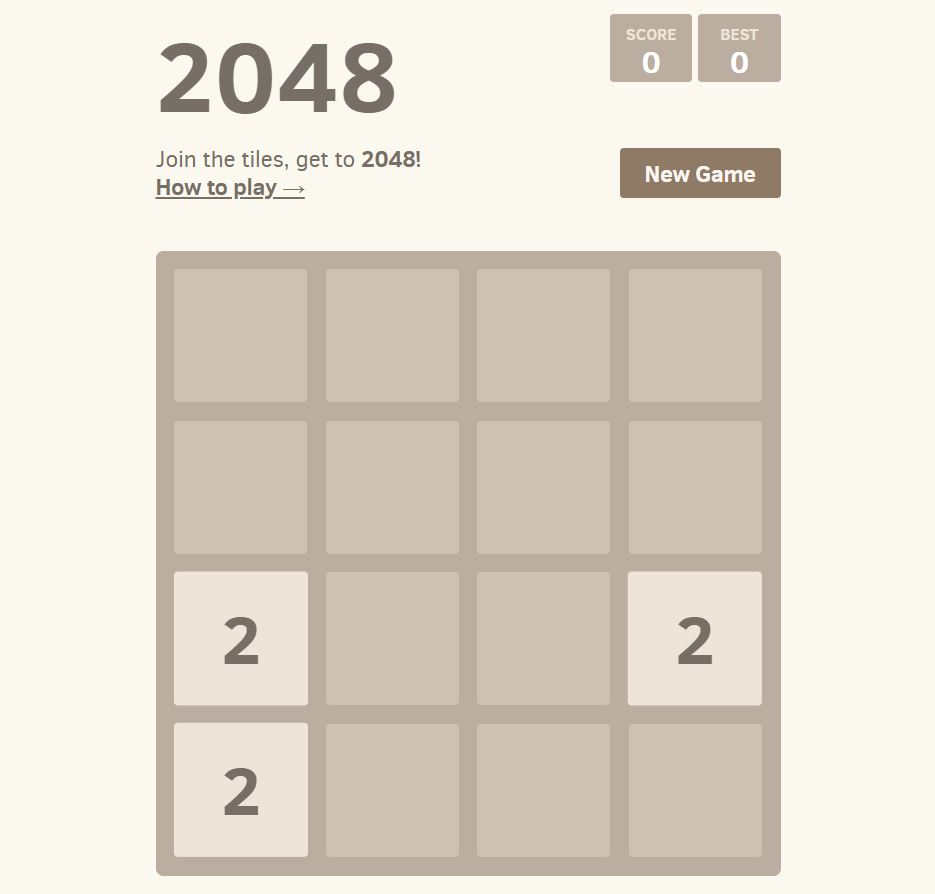
\includegraphics[width=0.9\linewidth, height=6cm]{originalni_2048_2}
			\caption{Potez u lijevo}
		\end{subfigure}
		
		\caption{Prikaz originalne igre \textit{2048} \cite{2048official}}
	\end{figure}
\newpage 
Potezima se svi postojeći elementi pomaknu u željenu stranu koliko i ako mogu, tj. ako im prazan prostor ili drugi elementi to dopuštaju. Primjer poteza može se vidjeti na slikama 2.1(a) i 2.1(b). Ako se dva ista kvadrata nađu jedan drugome na putanji spojit će se i proizvesti novi kvadrat s brojem jednakim zbroju brojeva u kvadratu. Spoj dva kvadrata s vrijednosti 2 prikazan je na slici 2.2.\newline
\begin{figure}[h]
	\centering
	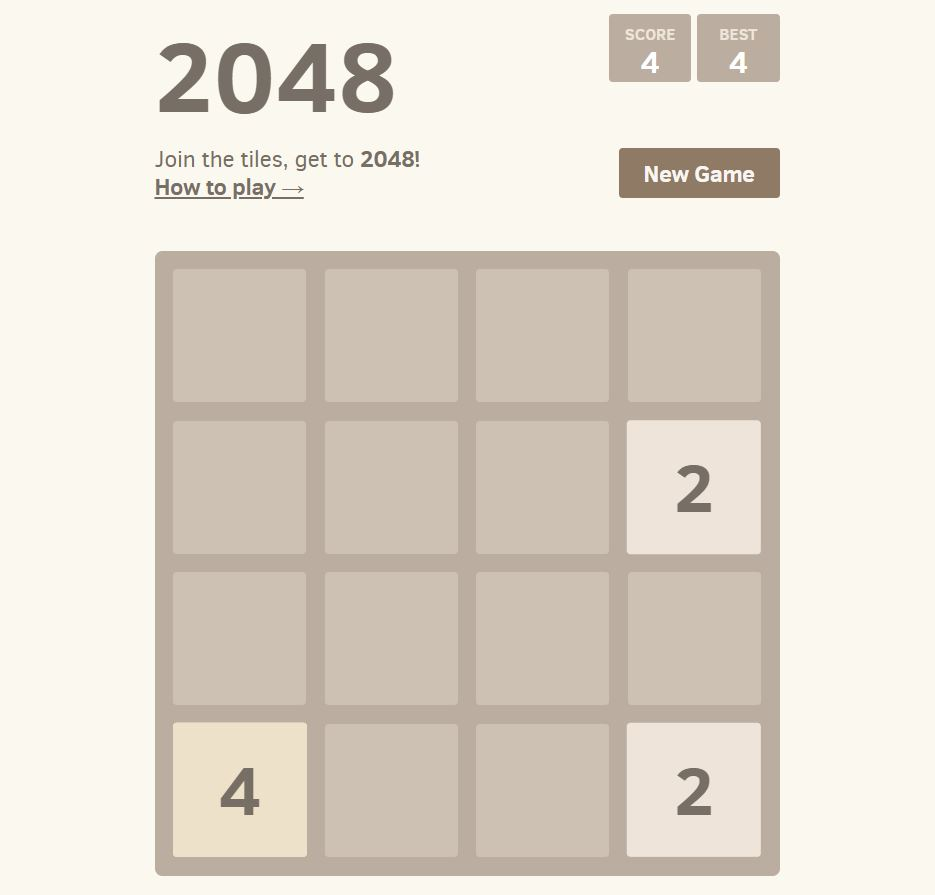
\includegraphics[width=0.5\linewidth]{originalni_2048_spajanje}
	\caption{Potez prema dolje, spajanje 2 i 2 \cite{2048official}}
\end{figure}
 \par
Potezi se ostvaruju pritiskom i puštanjem tipki strelica koje signaliziraju u kojem smjeru želimo pomaknuti sve elemente (gore,dolje,lijevo,desno). Potez se neće izvesti ako se njegovim izvođenjem neće izvesti nikakva promjena ploče, tj. nijedan element se neće pomaknuti zbog otpora drugog elementa ili ruba ploče. Držanjem strelice se postiže nekoliko rapidnih poteza u tom smjeru. Potezi prestaju otpuštanjem tipke ili ako se tim potezom neće pomaknuti niti jedan element. Kraj igre, Slika 2.3, nastaje ako imamo punu ploču i program prepozna da nijednim potezom nećemo postići promjenu rasporeda elemenata.\newline
\begin{figure}[h]
	\centering
	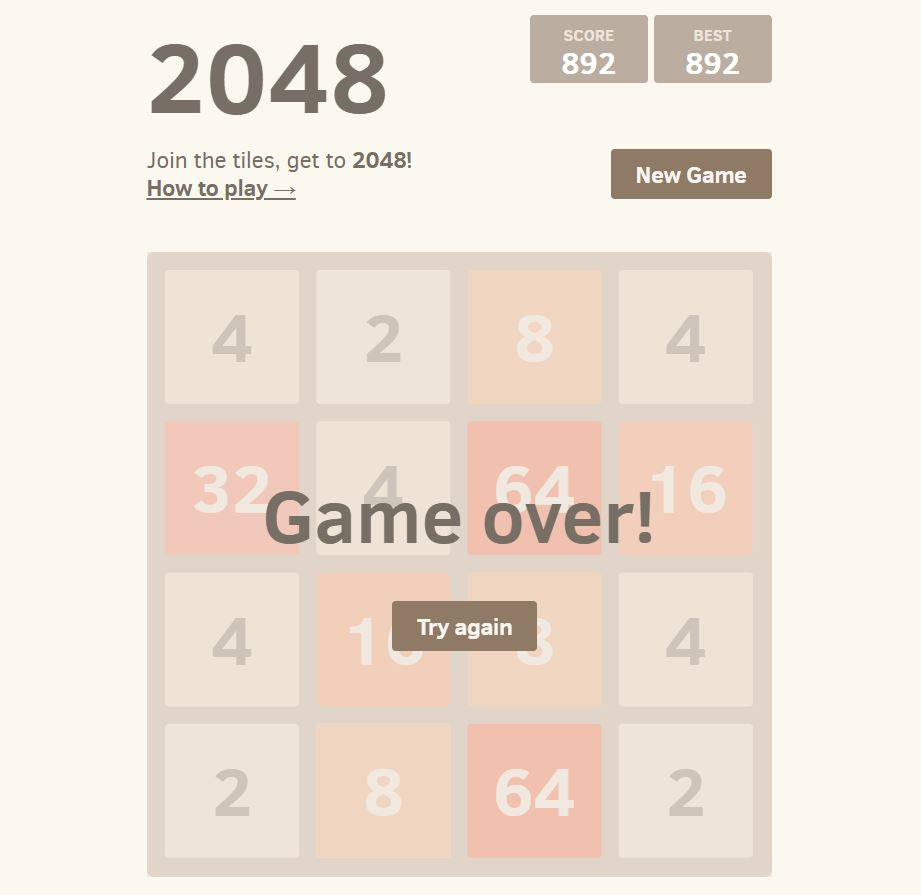
\includegraphics[width=0.5\linewidth]{originalni_2048_end}
	\caption{Kraj igre \cite{2048official}}
\end{figure}
\par
 Ako se dogodi da u jednom redu ili stupcu imamo poredak poput:
 \textbf{[2 2 4 8]} i napravimo potez u desno, dobit ćemo red: \textbf{[- 4 4 8]}. Dakle spajanje novih elemenata u potezu u kojem su napravljeni nije moguće. Ako imamo red oblika: \textbf{[2 2 4 4]}, potezom u desno dobivamo: \textbf{[- - 4 8]}. Višestruko spajanje elemenata je moguće te je omogućeno pomicanje u nove praznine u istom potezu.


\section{Verzija igre korištena u radu}
\quad Iako se ovaj rad referencira na originalnu igru, sam rad i njegova implementacija rađena je nad verzijom koja se po nekoliko elemenata razlikuje od originalne igre \textit{2048}.\par
Korištena verzija sadrži sljedeće grafičke elemente: ploča dimenzija 4x4, kvadrati raznih boja koji sadrže brojeve (potencije broja 2) te se nalaze na ploči, brojač koji prikazuju trenutni rezultat. Elementi se mogu vidjeti na slikama 2.4 i 2.5.
\par 
Prva bitna razlika u korištenoj verziji je ta da je rezultat zbroj brojeva na ploči, a ne zbroj brojeva u elementima koje je igrač dobio spajanjem. Iako je funkcionalnost donekle slična kao u početnoj verziji, vrijednost se više ne pripisuje igračevoj sposobnosti spajanja već se pripisuje količini i veličini brojeva na ploči.\newpage
\begin{figure}[h]
	\begin{subfigure}{0.5\textwidth}
		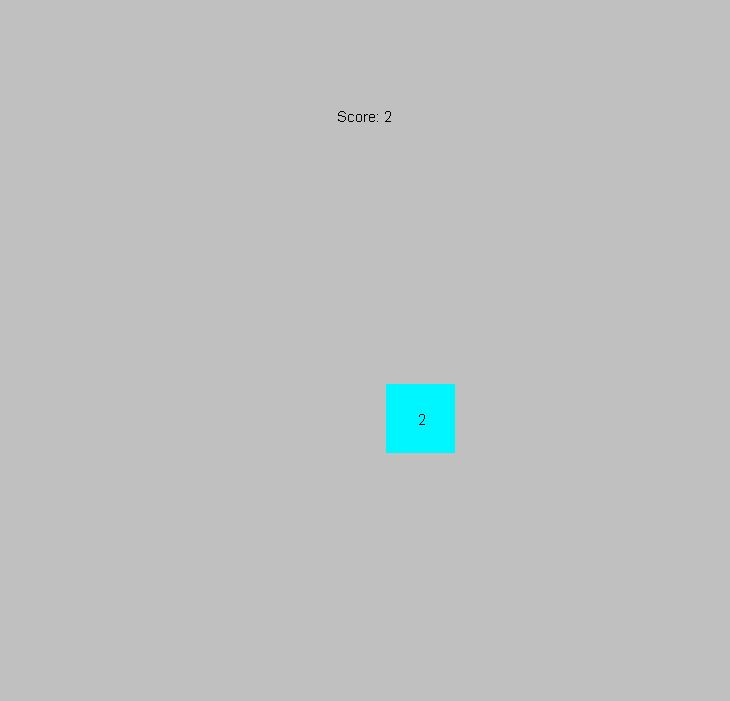
\includegraphics[width=0.9\linewidth, height=6cm]{nas_2048} 
		\caption{Početno stanje}
	\end{subfigure}
	\begin{subfigure}{0.5\textwidth}
		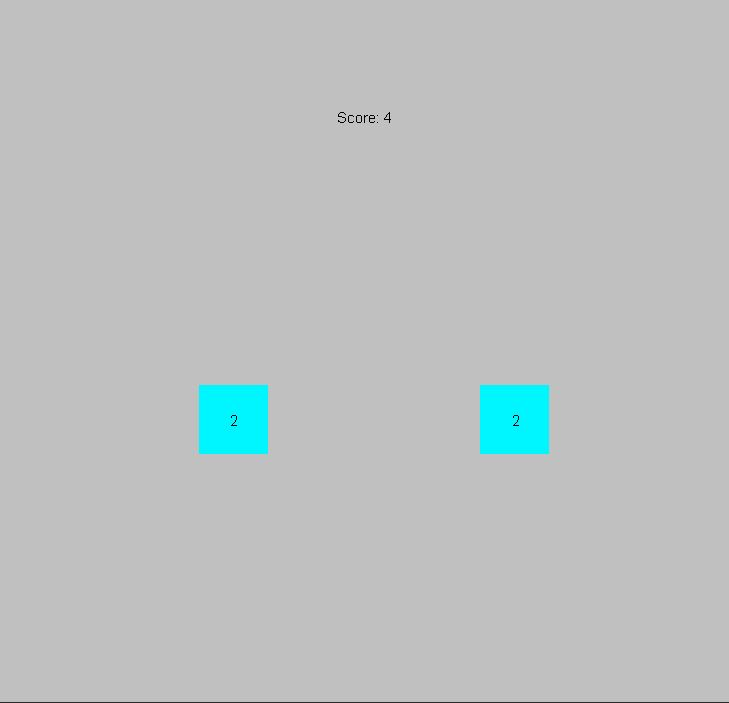
\includegraphics[width=0.9\linewidth, height=6cm]{nas_2048_2}
		\caption{Potez u lijevo}
	\end{subfigure}
	
	\caption{Prikaz korištene igre \textit{2048}}
\end{figure} 
Kretanja, ograničenja i spajanja elemenata na ploči slijede ista pravila kao i u originalnoj verziji igre.\newline
\begin{figure}[h]
	\centering
	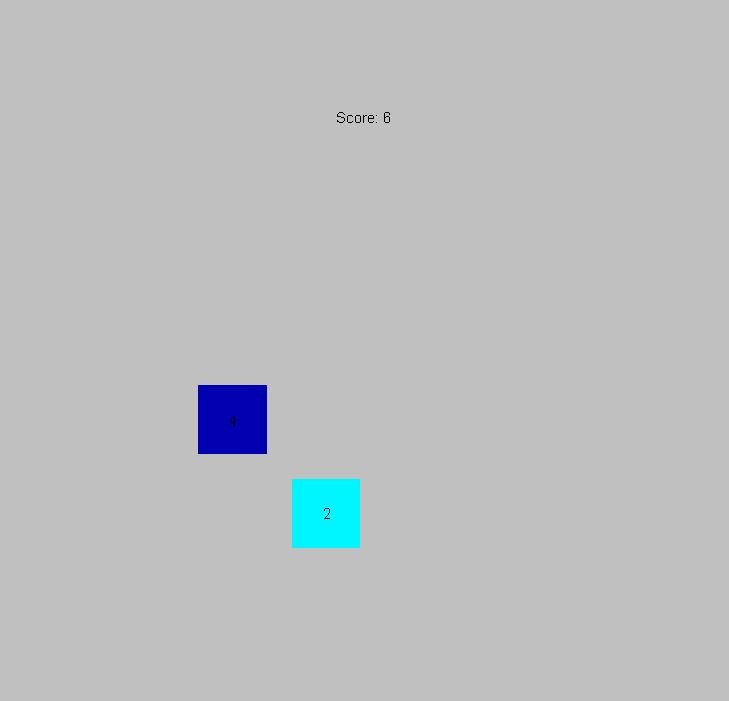
\includegraphics[width=0.5\linewidth]{nas_2048_spajanje}
	\caption{Potez prema lijevo, spajanje 2 i 2}
\end{figure}
\par
Potezi se ostvaruju pritiskom i \textbf{držanjem} tipki strelica koje signaliziraju u kojem smjeru želimo pomaknuti sve elemente. Ako se strelica ne drži do prestanka pomicanja svih elemenata postoji šansa da se igra počne nepredvidivo ponašati. Puštanje tipke strelice smatra se da je potez završio, a igra stvara novi element na nasumičnom slobodnom mjestu. Potezi će se izvesti čak iako se ne pomakne nijedan element. Kraj igre nastaje kad se pokuša dodati još jedan element na punu ploču.\par 
Ako se dogodi da u jednom redu ili stupcu imamo poredak poput:
\textbf{[2 2 4 8]} i napravimo potez u desno, dobit ćemo red: \textbf{[- - - 16]}. Dakle spajanje novih elemenata u potezu u kojem su napravljeni je moguće. Ako imamo red oblika: \textbf{[2 2 4 4]}, potezom u desno dobivamo: \textbf{[- - 4 8]}. Višestruko spajanje elemenata je moguće te je omogućeno pomicanje u nove praznine u istom potezu.\par 
Funkcioniranje verzije ovisi o grafičkom sučelju, a to stavlja veliko ograničenje na brzinu igranje igre. Potencijalna poboljšanja su smanjenje ovisnosti o grafičkom sučelju i promjena načina izvođenja poteza. To bi značilo da grafičko sučelje postane reprezentacija stanja koje je u pozadini, a ne ključni dio funkcioniranja igre, te da se potezi izvode na pritisak i puštanje tipki, a ne na držanje tipki.





\chapter{Genetsko programiranje}
\quad U ovom poglavlju dajemo uvid u osnove genetskog programiranja, a kasnije poglavlje će dati detaljan uvid u posebnu vrstu genetskog programiranja koja je korištena u radu. To je razlog zašto u ovom poglavlju nećemo ulaziti u najmanje detalje već ćemo se samo dotaknuti ključnih pojmova i operacija vezanih za područje genetskog programiranja.\par
Genetsko programiranje je tehnika evolucijskog algoritma koji automatski rješava probleme bez potrebe za tim da korisnik unaprijed zna ili odredi strukturu rješenja \cite{fieldguidtoGP}. \par 
Ključni koraci genetskog programiranja mogu se svesti na sljedeće:
\begin{algorithm}
	\caption{Genetsko programiranje \cite{fieldguidtoGP}}
	\begin{algorithmic}
		\State Stvori nasumičnu početnu populaciju programa pomoću danih funkcija, varijabli i konstanti
		\Repeat 
		\State Pokreni svaki program i dodjeli mu dobrotu
		\State Odaberi jednog ili dvoje roditelja na osnovu odabranog načina selekcije
		\State Stvori novi ili nove programe primjenjujući genetske operacije s određenom 
		\State vjerojatnošću
		\Until{Pronalazak zadovoljavajućeg rješenja ili ispunjenje nekog drugog uvjeta zaustavljanja (npr. dostignut maksimalan broj generacija)}\newline
		\Return Najbolji program
	\end{algorithmic}
\end{algorithm}\par 
U genetskom programiranju sve kreće od početne, često nasumične, populacije programa te se pokušava doći do što boljeg odgovora na početni zadatak kroz različite izmjene populacije tijekom generacija programa. 
\par 
Sintaksna stabla su čest oblik programa u genetskom programiranju. Unutarnje čvorove stabla čine funkcije, a njihova djeca postat će varijable koje ulaze u zadanu funkciju. Terminalni čvorovi (listovi) su konstante ili varijable nad kojima će se provesti funkcije sadržane u unutarnjim čvorovima. Primjer programa u obliku sintaksnog stabla možemo vidjeti na slici 3.1.\par
\begin{figure}[h]
	\centering
	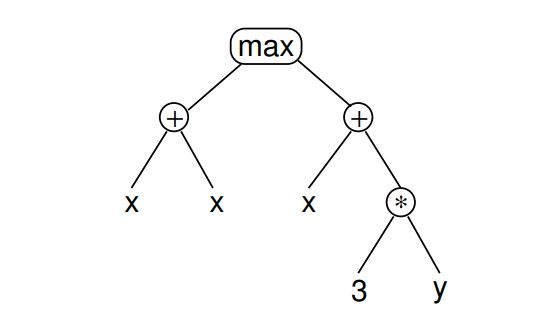
\includegraphics[width=0.5\linewidth]{fgtGP_tree}
	\caption{Sintaksno stablo (program) \cite{fieldguidtoGP}}
\end{figure}
 \par 
 Promjene su ključan dio razvoja programa, ali kao i u prirodi, promjene su nasumične i ne možemo garantirati da svaka promjena dovodi k boljem rješenju. Nasumičnost ima i svoje jače strane te često dovodi do novih i neočekivanih rješenja koja zaobilaze uobičajene poteškoće na koje nailaze determinističke metode \cite{fieldguidtoGP}. \par 
Prije uvođenja promjena vrši se selekcija. \textbf{Selekcija} je proces odabira roditelja uz pomoć kojih će se, kroz genetske operacije, uvesti novi programi u populaciju. U kasnijem poglavlju detaljnije ćemo opisati različite načine na koje se selekcija može izvesti. Bitno je da roditelji imaju veću šansu biti odabrani što su prilagođeniji našem zadatku. Osim toga, važno je dati mogućnost odabira manje prilagođenijih programa jer oni mogu sadržavati dijelove koji će dati bolje rezultate za generalni zadatak. 
\par 
Promjene između generacija događaju se zbog dvije ključne genetske operacije: 
\begin{itemize}
	\item \textbf{Križanje} (eng. \textit{Crossover}): Stvaranje novog programa/djeteta kombiniranjem nasumičnih dijelova roditeljskih programa
	\item \textbf{Mutacija} (eng. \textit{Mutation}): Stvaranje novog programa/djeteta nasumičnim mijenjanjem dijelova roditeljskog programa
\end{itemize}
\par
Oblik stabla čini križanje i mutaciju jednostavnijim i intuitivnijim. 
	\begin{figure}[h]
		\centering
		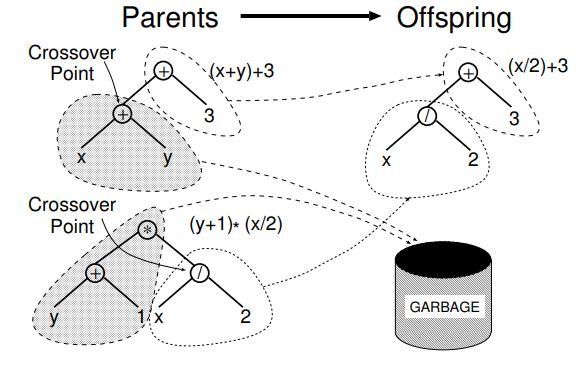
\includegraphics[width=0.7\linewidth]{fgtGP_crossover} 
		\caption{Križanje dviju kopija roditeljskih programa \cite{fieldguidtoGP}}
	\end{figure}
\newpage
\par
Križanje (Slika 3.2) možemo shvatiti kao miješanje i/ili zamjenu podstabala roditeljskih programa. Mutaciju (Slika 3.3) možemo shvatiti kao promjenu čvora gdje promjena može biti u obliku promjene funkcije/varijable na mjestu mutacije ili dodavanja u potpunosti novog podstabla na mjesto mutacije.\newline
	\begin{figure}[h]
		\centering
		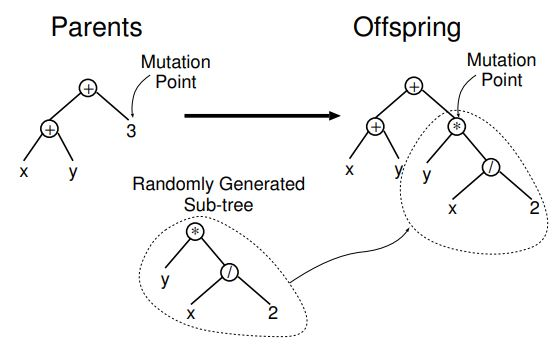
\includegraphics[width=0.7\linewidth]{fgtGP_mutation}
		\caption{Mutiranje roditelja dodavanjem novog podstabla na mjesto mutacije \cite{fieldguidtoGP}}
	\end{figure}
\par 
Napredak pojedinih programa prati se kroz generacije preko funkcije \textbf{dobrote}. \textbf{Dobrota} (eng. \textit{fitness}) je vrijednost koja ukazuje na to koliko je neki program dobar ili loš u rješavanju danog zadatka. Način računanja dobrote ovisni o tipu zadatka kojeg imamo te se prema tome može računati na različite načine.\par 
Dobrota nas dovodi do pojma elitizma u kojem ona igra glavnu ulogu. \textbf{Elitizam} je strategija kojom uspoređujemo dobrote programa unutar generacije te najbolji ili nekoliko najboljih programa trenutne generacije prebacujemo u sljedeću generaciju. Imamo veliku korist od ovakve strategije jer sprječava da najbolji program generacije bude lošiji od najboljih programa prošlih generacija. Sprječavamo nazadovanje kroz generacije.\par
Na kraju, mora postojati i \textbf{uvjet zaustavljanja} koji će reći da nema potrebe za daljnjim generacijama. \textbf{Uvjet zaustavljanja} može biti određena vrijednost dobrote ili dostizanje određenog broja generacija, ali može biti i neki drugi specifičan uvjet. 

	


\chapter{Kartezijevo genetsko programiranje}
\quad Kartezijevo genetsko programiranje (nadalje poznato kao CGP) oblik je genetskog programiranja koji je korišten u radu. Ovo poglavlje proći će kroz detalje koje ga čine posebnim i koji su bili bitni pri implementaciji. Osnove genetskog programiranja prenose se, ali u nešto drukčijim oblicima koji će se obraditi u sljedećim poglavljima.\par 
\section{CGP Mreže} 
\quad U Kartezijevom genetskom programiranju programi su prikazani kao dvodimenzionalne mreže čvorova. Mreža (Slika 4.1) je sastavljena od \textbf{c stupaca} i \textbf{r redova} koji dolaze uz \textbf{n ulaza} (eng. \textit{inputs}) i \textbf{m izlaza} (eng. \textit{outputs}).\newline
\begin{figure}[h]
	\centering
	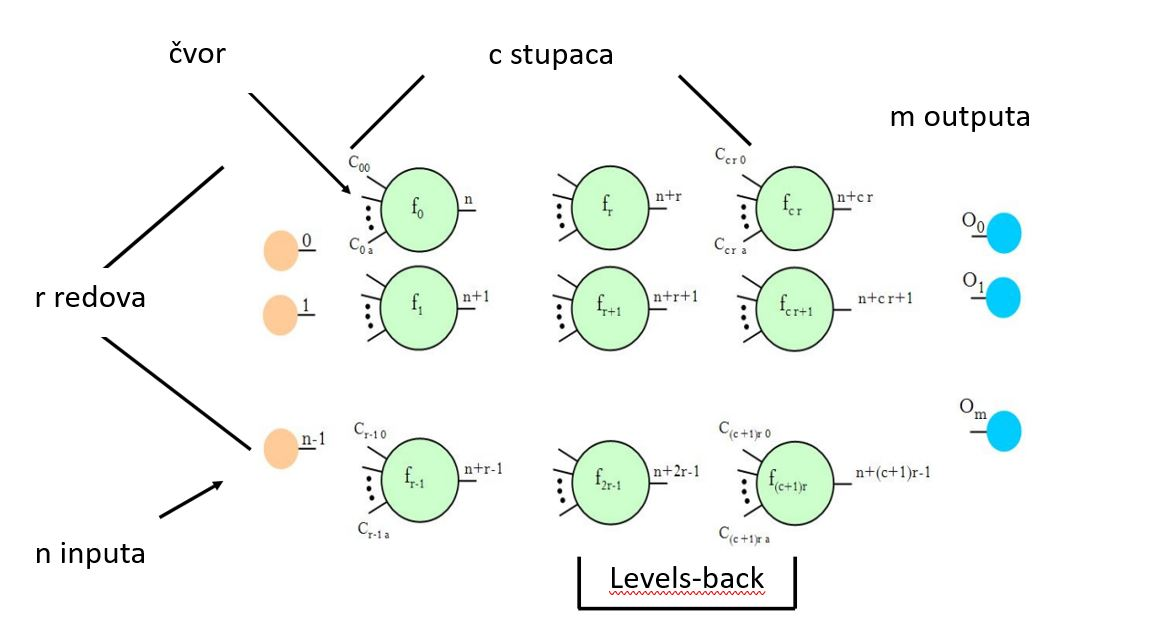
\includegraphics[width=0.9\linewidth]{cgp_mreza}
	\caption{CGP mreža \cite{CGPpresentation}}
\end{figure}  
\par 
Ovisno o broju stupaca i redova koje zadamo možemo imati različite oblike mreža. Možemo imati široke i plitke mreže (Slika 4.2 (a)), možemo imati uske i duboke mreže (Slika 4.2 (b)) ili možemo imati jednostavnu "kvadratnu" mrežu s jednakim brojem stupaca i redova.
\begin{figure}[h]
	\begin{subfigure}{0.5\textwidth}
		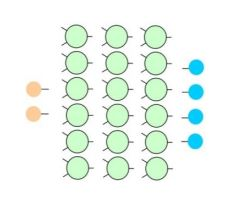
\includegraphics[width=0.9\linewidth]{cgp_wide} 
		\caption{Široka i plitka mreža \cite{CGPpresentation}}
	\end{subfigure}
	\begin{subfigure}[b]{0.5\textwidth}
		\raisebox{1.25cm}{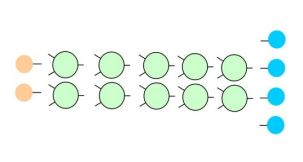
\includegraphics[width=0.9\linewidth]{cgp_deep}}
		\caption{Uska i duboka mreža \cite{CGPpresentation}}
	\end{subfigure}
	
	\caption{Mogući oblici CGP mreža}
\end{figure}
\newpage
\par Oblik i veličina mreže trebali bi biti prilagođeni zadatku s obzirom na to da premala ili prevelika mreža mogu biti izvor problema ili slabog treniranja programa. Jedna od preporučenih i zanimljivijih mreža je mreža s jednim redom i proizvoljnim brojem stupaca koja više nalikuje lancu. U ovom radu najviše se radilo s ovakvim oblikom mreže, a primjer oblika može se vidjeti na slici 4.3.

\begin{figure}[h]
	\centering
	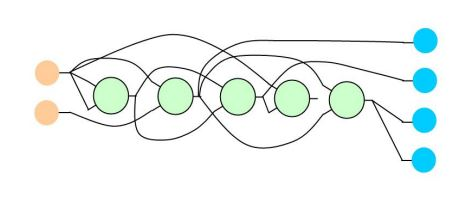
\includegraphics[width=0.9\linewidth]{cgp_chain}
	\caption{CGP mreža s jednim redom \cite{CGPpresentation}}
\end{figure}
\section{Čvorovi mreže}
\par 
 \quad Čvorovi su sastavljeni od gena koji tvore genotip, a zapravo su brojevi koji sugeriraju od kuda će čvor dobiti podatke, koje operacije će primijeniti nad podacima i od kud će doći izlazni podaci \cite{CGPbook}. 
 \par Veze između čvorova upravo su geni veza i oni nam govore iz kojeg ćemo čvora ili ulaza dobiti podatke. Broj gena veza koje sadrži svaki čvor mreže jednak je najvećem broju parametara koje traži neka od funkcija koja se može pojaviti u mreži. Pošto su svi čvorovi i ulazi numerirani ti brojevi su nam adrese. Geni veza najčešće mogu sadržavati samo adrese čvorova i ulaza iz stupaca s lijeve strane čvora za koji se adresiraju ulazni parametri, ali postoje radovi i primjeri gdje se dopuštaju ciklusi (ciklički CGP) micanjem ove restrikcije \cite{CGPbook}. Parametar \textit{\textbf{Levels-back (l)}} govori nam iz kojih stupaca s lijeve strane trenutne pozicije možemo uzeti adresu. Primjerice za \textit{l} = 1 adrese možemo uzimati samo iz lijevog neposrednog stupca. Za \textit{l} = $ n_{c} $ (l = broj stupaca) možemo dohvatiti bilo koju adresu iz mreže u bilo kojem stupcu.
 \par 
Sve funkcije koje se mogu pojaviti u čvorovima zapisane su u posebnu tablicu uz svoju brojevnu reprezentaciju. Brojevna reprezentacija postaje adresa funkcije i ona se zapisuje kao funkcijski gen koji je ključni dio svakog čvora mreže. Nakon što čvor dobije potrebne parametre preko gena veza, dohvaća se funkcija pod zadanom adresom i ona se izvršava nad danim parametrima.
\par
Izlazni geni nalaze se na krajnjoj desnoj strani mreže. Oni adresiraju čvorove ili ulaze iz kojih će se uzimati vrijednosti za konačni izlaz iz mreže. Za njih vrijede ista pravila kao i za gene veza. Na osnovu izlaza iz mreže poduzima se akcija jedinstvena za taj izlaz, čineći izlaz iz mreže odlukom mreže.\par 
Primjer mreže čvorova sa zadanim genima i vezama možemo vidjeti na slikama 4.4. i 4.5. uz funkcije u tablici 4.1.
\begin{figure}[h]
	\centering
	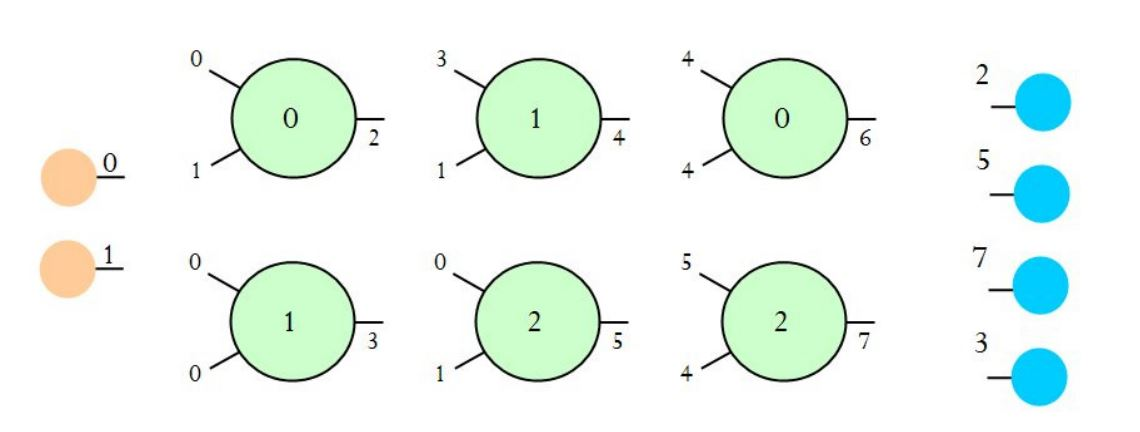
\includegraphics[width=0.9\linewidth]{cgp_mreza_zadana_a}
	\caption{CGP mreža s genima \cite{CGPpresentation}}
\end{figure}
\begin{figure}[h]
	\centering
	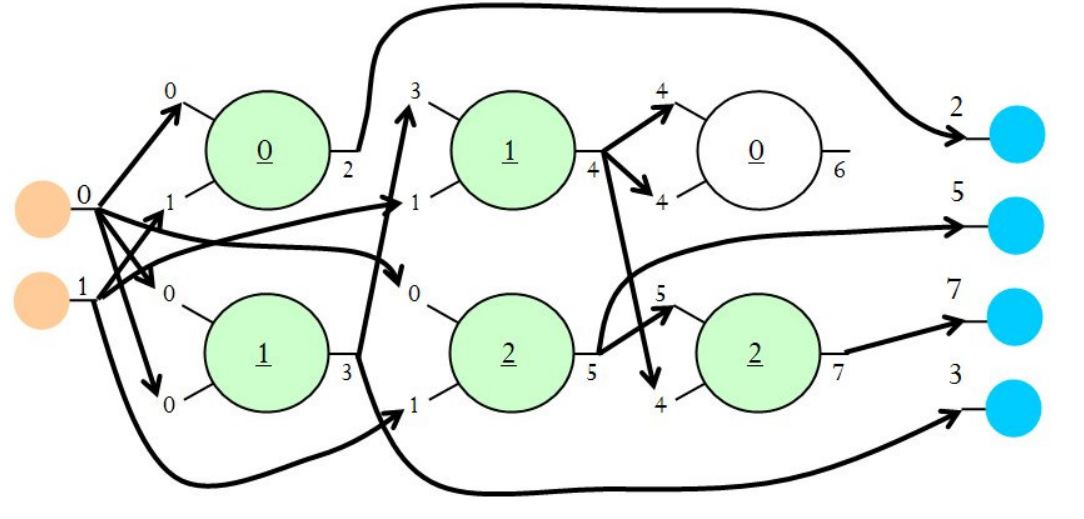
\includegraphics[width=0.9\linewidth]{cgp_mreza_zadana_b}
	\caption{CGP mreža s genima i vezama \cite{CGPpresentation}}
\end{figure}
\begin{table}[h!]
\centering
\begin{tabular}{ |c|c|c|c|  }
	\hline
	0 & 1 & 2 & 3\\
	\hline
	+ Zbroji parametre  & - Oduzmi parametre &
	* Pomnoži parametre & / Podijeli parametre\\
	\hline
\end{tabular}
\caption{Tablica funkcija (Lookup table of functions)}
\end{table}
\section{Genotip i fenotip}
\par 
\quad Pogledom na sliku 4.3. uviđamo kako je gen u trećem stupcu i prvom retku nekorišten, tj. on ne pridonosi niti jednom izlazu. On se naziva \textit{nekodirajućim genom}. Dolazimo do pojmova \textbf{genotipa} i \textbf{fenotipa}. \textit{"Dekodiranje genotipa rezultira programom koji se naziva fenotip \cite{CGPbook}."} \quad \textbf{Genotip} čine svi geni unutar mreže dok \textbf{fenotip} čine samo aktivni,\textit{ kodirajući}, geni koji utječu na izlaze iz mreže. U većim mrežama broj nekodirajućih gena može biti znatno veći od broja kodirajućih. Primjerice J. F. Miller i S. L. Smith pokazali su kako je u genotipu s 4000 čvorova postotak nekodirajućih čvorova oko 95\% \cite{geneticredundancy}. 
\par
Dekodiranje genotipa naziv je za proces kojim ćemo proći kroz genotip i utvrditi koji geni su kodirajući, a koji ne. Princip procesa je krenuti od izlaznih gena i kretati se po čvorovima čije adrese se nalaze u genima veza dok ne dođemo do ulaza u mrežu. Pseudokodom u Algoritmu 2 prikazan je proces dekodiranja.

\begin{algorithm}
	\caption{Dekodiranje genotipa}
	\begin{algorithmic}
		\State Lista čvorova
		\For{svaki izlazni gen}
		\If{adresa = adresa čvora}
		\State Označi čvor kao kodirajući
		\EndIf 
		\EndFor
		\For{svaki čvor u \textit{Lista čvorova} krenuvši od zadnjeg}
		\If{čvor je kodirajući}
		\For{gen veze u čvoru}
		\If{adresa = adresa čvora}
		\State Označi čvor kao kodirajući
		\EndIf 
		\EndFor
		\EndIf
		\EndFor\newline
		\Return Lista čvorova
	\end{algorithmic}
\end{algorithm}
\newpage
\section{CGP kao niz brojeva}
\par 
\quad Tijekom opisa Kartezijevog genetskog programiranja susreli smo se već nekoliko puta s brojevima i brojevnom reprezentacijom, a svi brojevi zapravo su adrese. Upravo zbog tih brojeva postoji vrlo jednostavan zapis genotipa i to u obliku niza brojeva. U tom nizu moramo znati raspoznati gene - funkcijski geni, geni veza i izlazni geni. Iako u nizu nećemo imati nikakvu posebnu reprezentaciju znat ćemo točno koji je gen koji ako znamo koliko parametara svaki čvor treba primiti i koliko izlaza imamo. Uzmemo li mrežu na Slici 4.4 kao primjer, možemo konstruirati reprezentaciju mreže krenemo li od gornjeg lijevog čvora: \newline

\makebox[\textwidth][c]{%
	\begin{minipage}{0.1\textwidth}
		\par \textbf{\underline{0} 0 1}
\end{minipage}}\newline
\par 
U čitanje niza ulazimo sa znanjem da je najveći broj parametara potreban nekoj od mogućih funkcija dva te da imamo dva izlaza iz mreže. Slijeva nadesno imamo: funkcijski gen s brojem \textit{0} koji adresira funkciju zbrajanja u tablici funkcija (Tablica 4.1), prvi gen veze koji adresira od kud dobivamo prvi parametar što bi u ovom primjeru bio \textit{0} - prvi ulaz/input, drugi gen veze koji adresira od kud dobivamo drugi parametar što bi u ovom primjeru bio \textit{1} - drugi ulaz/input. Nastavimo li dalje prolaziti po čvorovima dobivamo sljedeći niz: \newline

\makebox[\textwidth][c]{%
	\begin{minipage}{0.7\textwidth}
		\par \textbf{\underline{0} 0 1  \quad\underline{1} 0 0  \quad\underline{1} 3 1  \quad\underline{2} 0 1  \quad\underline{0} 4 4  \quad\underline{2} 5 4  \qquad 2 5 7 3}
\end{minipage}}\newline
\par
Pogledamo li u nizu treći čvor vidimo kako njegov prvi gen veze sadrži broj \textit{3}. Pošto imamo samo dva ulaza i njihove adrese su \textit{0} i \textit{1} to znači kako je adresiran jedan od čvorova; u ovom slučaju drugi čvor u prvom stupcu. Prema tome, adrese čvorova nastavljaju se na adrese ulaza jer oni sami postaju ulazi za neki sljedeći čvor ili izlaz. Adrese se povećavaju s lijeva nadesno i od vrha stupca prema dnu stupca.\par
Zadnji dio niza koji je ovdje posebno odvojen od ostatka niza čine izlazni geni. U ovom slučaju na izlaz iz mreže spojeni su prvi, drugi, četvrti i šesti čvor. \par
Ovakav oblik CGP mreže/programa izuzetno je koristan i pojednostavljuje inicijalizaciju, izvršavanje i promjenu programa. Promjene nad populacijom i pojedinim programima obrađuju se kasnije u zasebnim poglavljima.\par 

\section{Inicijalizacija programa/populacije}
 \quad Inicijalizacija, kao i u običnom genetskom programiranju, podrazumijeva stvaranje nasumične populacije programa. U ovom slučaju to bi bili nizovi nasumičnih brojeva. \par 
 Iako brojevi jesu nasumični, postoje pravila koja smo ranije postavili i koja moramo poštivati. Nizovi moraju biti smisleni i slijediti formu sličnoj onoj iz primjera gdje znamo na kojim mjestima se nalaze funkcijski geni, na kojima geni veza i na kojima izlazni geni. Osim forme, adrese koje se mogu pojaviti na određenim pozicijama moraju biti ograničene na isti način kao u mreži. Funkcijski geni smiju imati samo adrese iz tablice funkcija, ali te adrese mogu se pojaviti u bilo kojem dijelu niza gdje se nalaze funkcijski geni. Geni veza (osim ako se radi o cikličkom CGP-u) smiju imati samo adrese čvorova iz stupaca lijevo od njihovog stupca, naravno s danim ograničenjem Levels-back. Informaciju o tome u kojem se stupcu nalazi koji čvor dobivamo iz kombinacije informacija: broj redova mreže, tj. koliko čvorova imamo u svakom stupcu, i praćenjem rednog broja čvora u kojem se nalazimo. Izlazni geni smiju sadržavati adrese svih čvorova i ulaza u mreži.  \par 
 Slijedeći ova pravila možemo inicijalizirati cijelu populaciju programa jednostavnog zapisa u kratkom roku.\newpage \par U nastavku možemo vidjeti jednu takvu populaciju mreža koje imaju šesnaest ulaza, četiri izlaza, širinu jedan, dubinu osam i maksimalan broj parametara funkcija dva. Radi preglednosti nizovi su podijeljeni na čvorove i izlaze, funkcijski geni su \underline{podcrtani}, a izlazni geni su \textbf{podebljani}.\newline
 
\begin{table}[h!]
\centering
\begin{tabular}{ |c|c|c|c|c|c|c|c|c|  }
	\hline
	\underline{4} 6 14 & \underline{5} 15 16 & \underline{4} 0 8 & \underline{4} 15 15 & \underline{2} 8 3 & \underline{4} 7 10 & \underline{1} 17 3 & \underline{3} 13 3 & \textbf{13 23 4 10}\\
	\hline
\end{tabular}
\end{table}

\begin{table}[h!]
	\centering
	\begin{tabular}{ |c|c|c|c|c|c|c|c|c|  }
		\hline
	 \underline{4} 14 5 & \underline{3} 15 6 & \underline{5} 1 7 & \underline{4} 7 12 & \underline{2} 0 15 & \underline{1} 19 3 & \underline{1} 16 9 & \underline{0} 14 3 & \textbf{20 22 1 11} \\
		\hline
	\end{tabular}
\end{table}

\begin{table}[h!]
	\centering
	\begin{tabular}{ |c|c|c|c|c|c|c|c|c|  }
		\hline
		\underline{4} 14 7 & \underline{3} 1 4 & \underline{5} 13 11 & \underline{1} 15 1 & \underline{2} 6 2 & \underline{4} 12 9 & \underline{1} 1 13 & \underline{5} 12 3 & \textbf{7 23 20 20}\\
		\hline
	\end{tabular}
\end{table}

\begin{table}[h!]
	\centering
	\begin{tabular}{ |c|c|c|c|c|c|c|c|c|  }
		\hline
		\underline{2} 15 8 & \underline{1} 2 7 & \underline{2} 17 9 & \underline{1} 4 15 & \underline{3} 8 1 & \underline{5} 6 18 & \underline{2} 19 10 & \underline{3} 14 19 & \textbf{0 5 10 21}\\
		\hline
	\end{tabular}
\end{table}

  
 
\section{Izvođenje programa}  
\quad Sad kad smo upoznati s oblikom programa i pojmom fenotipa možemo govoriti o izvođenju programa. Prije izvođenja programa potrebno ga je dekodirati kako bi radili samo s onim čvorovima koji nam utječu na izlaz iz mreže. Nakon što smo dobili fenotip, počinjemo s procesom koji je po prolazu kroz mrežu obrnut od dekodiranja. Pod pretpostavkom da radimo s necikličnom mrežom, imamo unaprijednu (eng. feed-forward) mrežu koja obrađuje i propagira podatke od ulaza prema izlazu. Izvođenje programa se zbog toga odvija stupac po stupac od ulaza prema izlazu kako ni u jednom trenutku ne bi došli do čvora koji ima nedefinirane ulazne parametre. Za svaki čvor slijedimo njegove gene veza do parametara koje uvrštavamo u funkciju adresiranu u funkcijskom genu. Rezultat funkcije zapamtimo kao izlaz iz čvora. Nastavljamo dalje čvor po čvor dok ne dođemo do izlaznih gena koji dohvaćaju izlaze čvorova ili ulaze u mrežu. \par
Ovime smo pokrenuli i izvršili program koji smo sastavili. Kao rezultat izvođenja programa dobili smo izlaz koji se može interpretirati kao odgovor na zadani zadatak ili dalje koristiti u svrhu rješavanja zadatka.

\chapter{Dobrota i selekcija}
\quad U ovom poglavlju zaći ćemo dublje u pojam dobrote i proces selekcije te predložiti nekoliko načina implementacije.

\section{Dobrota}
\quad U 3. poglavlju dotakli smo se pojma dobrote (eng. fitness) te dali kratki i jednostavan opis koji proširujemo ovdje. Dobrota je vrijednost koju koristimo kako bi mogli reći koliko je program dobar u rješavanju danog zadatka i koju koristimo pri međusobnom uspoređivanju različitih programa. Dobrota nema univerzalan način računanja niti univerzalan okvir vrijednosti, ali očekuje se da je program bolji u rješavanju zadatka što je dobrota veća.\par 
U nadziranom učenju naši programi, uz ulazne vrijednosti, dobivaju i očekivane izlazne vrijednosti. Očekivane izlazne vrijednosti služe za uspoređivanje s izlaznim vrijednostima naših programa. Usporedbom dobivamo pogrešku (eng. error) koja nam govori koliko se rezultati naših programa razlikuju od očekivanog izlaza. Pogrešku možemo koristiti kako bi izračunali dobrotu. Način pretvorbe pogreške u dobrotu ostavlja se na izbor osobi koja će implementirati nadzirano učenje, ali ovdje će se predložiti jedna jednostavna operacija. Operacija u pitanju je cjelobrojno dijeljenje broja jedan s pogreškom ($ \frac{1}{error} $). Operacija čini dvije vrijednosti obrnuto proporcionalne i u potpunosti je prihvatljiva opcija.\par 
U podržanom učenju naši programi dobivaju niz ulaznih vrijednosti prema kojima donose "odluke". "Odluke" se mogu ili kazniti ili nagraditi. Kazna i nagrada nisu odmah uočljivi što znači da se program neće ocijeniti pri primitku prve kazne/nagrade. Kazne i nagrade se akumuliraju kroz više "odluka". Primijenimo li primjer igre, naši programi će raditi poteze kroz runde i bit će kažnjeni ili nagrađeni za njih, a na kraju igre dobivaju konačan rezultat koji je procjena koliko su bili uspješni u igri. Ako se radi o zadatku u kojem postoje elementi nasumičnosti bilo bi dobro svaki program nekoliko puta provesti kroz zadatak kako bi se uvjerili da se uvjeti u zadatku nisu poklopili na takav način da program dobije upravo takvu procjenu uspješnosti.\par 
Elitizam je pojam koji smo obradili u 3. poglavlju. U tom poglavlju je pojam dovoljno dobro objašnjen i ovdje ćemo samo napraviti nadogradnju vezanu za CGP. Ako se utvrdi da roditelj i dijete imaju istu dobrotu, dijete će se propagirati u sljedeću generaciju \cite{CGPbook}\cite{CGPpresentation}. Testovima  je dokazano kako je propagacija djeteta u takvim slučajevima izuzetno korisna i efektivna u dobivanju boljih rezultata \cite{CGPbook}.
\par
Dobrota je izuzetno korisna, ali to ne znači da nas ne može zavarati. Problemi koje ćemo navesti nisu toliko vezani uz sam postupak dobivanja dobrote, oni mogu doći iz različitih dijelova sustava koji razvija programe, ali ti problemi utječu na dobrotu koja nas zatim može zavarati i potaknuti na krivi zaključak. Neki od problema koji se mogu vezati uz dobrotu su pretreniranost i nasumičnost zadatka.\par 
Pretreniranost možemo najviše povezati uz nadzirano učenje. Kod pretreniranosti možemo dobiti sjajne rezultate za podatke nad kojima učimo, ali loše rezultate za neviđeni skup podataka. Tu nas dobrota tehnički ne vara, programi sjajno rade na podskupu za učenje, ali programi ne znaju riješiti generalni tip zadatka. To se događa kad se naši programi previše razviju u smjeru rješavanja jako specifičnih zadataka. Posljedica toga je ta da se pretrenirani programi kroz elitizam i selekciju, zbog visoke dobrote, propagiraju dalje i pretreniraju buduće generacije. Problem se može spriječiti boljom generalizacijom skupa za učenje i ograničavanjem broja generacija ili dobrote.
\par
Pod nasumičnost zadatka misli se na problem koji se javlja kod podržanog učenja kad zadatak ima neke elemente nasumičnosti. Kao što je već ranije spomenuto ne znamo kako će se zadatak dalje razvijati i može se dogoditi da u ponavljanjima dođu izrazito teški ili izrazito laki zadaci. Primjerice, može nastupiti slučaj gdje generalno loš program uspješnije rješava svoje zadatka nego što generalno bolji program rješava svoje, a razlog tome je taj da su se nekoliko puta za redom poklopili posebni uvjeti koji su to omogućili. Posljedica ovog problema je propagacija lošijeg programa u sljedeće generacije. Rješenje ovom problemu može biti provođenje programa kroz zadatak više puta ili drukčiji pristup računanju dobrote.

\section{Selekcija}
\quad Selekciju smo spomenuli u 3. poglavlju, a ovdje ćemo ju dodatno obraditi i navesti neke načine implementacije.\par
 Selekcijom odabiremo programe (roditelje) koji će zajedno biti temelji za nove programe koji će se uvesti u sljedećim generacijama. Povlačimo poveznicu s prirodnim svijetom gdje najuspješnije jedinke dobivaju prioritet prilikom parenja i tako osiguravaju prenošenje svojih gena u buduću generaciju. No, kao i u prirodnom svijetu, ne moraju se samo najbolje jedinke pariti i prenositi svoje gene. To pridonosi raznolikosti unutar vrste, a same slabosti u jednoj situaciji mogu postati snage u drugoj. Po uzoru na opisan proces, imamo nekoliko načina na koje možemo implementirati selekciju.
 \par 
 Prvi i najjednostavniji način koji zahtijeva samo sortiranje programa po dobroti bio bi da uzmemo najbolje programe. Naravno varijante ove implementacije su itekako moguće: jedan najbolji program i jedan najlošiji; par programa s početka, par iz sredine i par s kraja sortiranog niza; jedan program s početka i jedan program iz sredine sortiranog niza... Učinkovitost ovakve selekcije upitna je i u ovom radu neistražena tako da se predlažu neki od sljedećih načina implementacije.\par 
 Selekcija proporcionalna dobroti može se zamisliti kao kotač s kazaljkom koji je podijeljen na dijelove. Svaki dio je reprezentacija jednog programa. Veličina dijela proporcionalna je udjelu dobrote programa u zbroju dobrota svih programa. Primjerice, ako zbrojimo dobrote četiri programa i ako je dobrota jednog program pridonijela trećini zbroja, njegov dio na kotaču pokrivat će jednu trećinu kotača.\newline
 \begin{figure}[h]
 	\centering
 	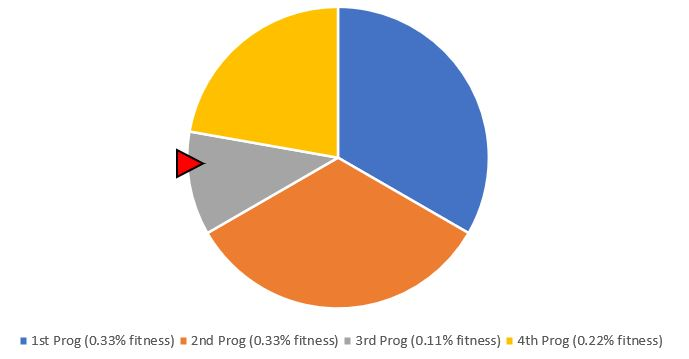
\includegraphics[width=0.9\linewidth]{proporcionalna_selekcija}
 	\caption{Vizualni prikaz selekcije proporcionalne dobroti}
 \end{figure}
 \par 
  Nakon što izračunamo udio svakog programa, nasumično odabiremo programe. Vjerojatnost odabira svakog programa jednaka je njegovom udjelu. Vizualiziramo li taj događaj, zavrtimo kotač i odaberemo program na koji pokazuje kazaljka nakon što se kotač zaustavi. Ovakav oblik implementacije selekcije pokazao se izrazito uspješnim i preporučuje se.
  \par
  Zadnji način implementacije selekcije koji ćemo opisati može biti nadogradnja prethodnom načinu, a naziva se turnir. Nakon što odaberemo nekoliko programa, sasvim nasumice ili po udjelu dobrote, uspoređujemo programe međusobno i najbolji postaju roditelji. Ovaj oblik implementacije daje priliku i slabijim programima jer oni trebaju biti najbolji samo u svojoj skupini, a ne u cijeloj populaciji programa.
  \par
  Selekcija nema nekih osobitih problema koje možemo popraviti. Uvijek postoji mogućnost da ćemo za roditelje odabrati slabije programe ili da će se često odabrati isti programi. Implementacijom gore navedenih strategija pokušava se smanjiti učestalost takvih situacija, a ipak zadržati raznolikost populacije. Ispravna implementacija strategija ključna je za ispravno funkcioniranje selekcije.
  \par
  Ako se tijekom selekcije u CGP-u dogodi slučaj gdje roditelj i dijete imaju istu vrijednost po kojoj se uspoređuju (npr. dobrota), a izbor je između jednog ili drugog, izabrat će se dijete zbog istog razloga koji je naveden za elitizam u prošlom potpoglavlju \cite{CGPbook}\cite{CGPpresentation}. 

\chapter{Križanje}
\quad Nakon što smo selekcijom dobili roditelje budućih programa, operacijom križanja pokušavamo stvoriti djecu ispreplećući roditeljske gene. U CGP-u ne radimo sa stablima već s mrežama što nas potiče na drukčiji pristup od onog opisanog u 3. poglavlju. U ovom poglavlju opisuje se križanje u CGP-u, utjecaj operacije na uspješnost programa i neki od načina implementacije.

\par
Križanje u CGP-u jako je zanimljiva tema. Tema koja se još uvijek istražuje i koja dobar dio vremena nije bila u fokusu. Primjenom operacije u nekim slučajevima dobivamo bolje rezultate nego kad se operacija ne primjenjuje, ali u nekim slučajevima i gore. Način implementacije znatno utječe na djelotvornost operacije \cite{CGPbook}\cite{CGPpresentation}. Zato se križanju, posebice u CGP-u, pristupa jako pažljivo i nerijetko se izbjegava. Križanje može biti snažan alat koji će spojiti najbolje dijelove roditelja ili alat koji će poremetiti ono što je roditelje činilo uspješnim.
\par
Originalni pokušaj ostvarenja križanja u CGP-u donekle je jednostavan. U mreži možemo odabrati nasumični gen te na mjestu odabranog gena presjeći obje kopije roditelja. Potom uzimamo prvi dio prve kopije i spajamo ga s drugim dijelom druge kopije, a zatim spajamo drugi dio prve kopije s prvim dijelom druge kopije. Vizualizaciju ovog procesa možemo vidjeti na slikama 6.1(a)-6.3(b).
\begin{figure}[h]
	\centering
	\begin{subfigure}{0.4\textwidth}
		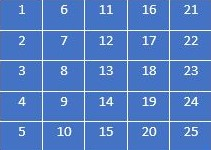
\includegraphics[width=0.9\linewidth]{cross_1} 
		\caption{Kopija prvog roditelja}
	\end{subfigure}
	\begin{subfigure}{0.4\textwidth}
		{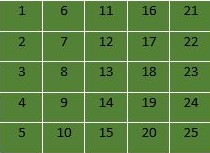
\includegraphics[width=0.9\linewidth]{cross_2}}
		\caption{Kopija drugog roditelja}
	\end{subfigure}
	\caption{Početne mreže roditelja }
\end{figure}

 \begin{figure}[h]
	\centering
	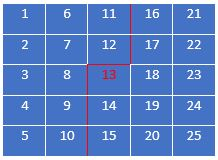
\includegraphics[width=0.4\linewidth]{cross_3}
	\caption{Odabir gena za presjek}
\end{figure}

\begin{figure}[h]
	\centering
	\begin{subfigure}{0.4\textwidth}
		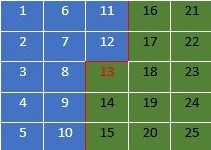
\includegraphics[width=0.9\linewidth]{cross_4} 
		\caption{Prvo dijete}
	\end{subfigure}
	\begin{subfigure}[b]{0.4\textwidth}
		{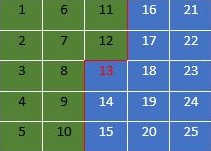
\includegraphics[width=0.9\linewidth]{cross_5}}
		\caption{Drugo dijete}
	\end{subfigure}
	\caption{Djeca nastala spajanjem dva dijela roditelja}
\end{figure}
\newpage
\par
Ovakav oblik križanja pokazao se izrazito destruktivnim u drugim radovima \cite{CGPbook}. Ipak, ovakav oblik križanja korišten je u ovom radu na mrežama širine jedan. Učinak takvog križanja na žalost nije provjeren u radu, križanje je provedeno u svim testovima. Ostavlja se kao potencijalna tema daljnjeg istraživanja. 
\par
Tijekom godina razvijeno je nekoliko drugih metoda među kojima se ističe metoda zamjene podgrafova aktivnih čvorova \cite{newcross}. Metoda je slična gore navedenoj metodi, ali ne dijelimo i ne spajamo sve gene grafa već samo one kodirajuće/aktivne što bi trebalo smanjiti destruktivnost i poremećaje u novim mrežama. 

\chapter{Mutacija}
\quad Križanjem nastaju djeca koja sadrže gene oba roditelja, ali konstantnim korištenjem istog genetskog materijala možemo postići samo određene rezultate. Mutacija nam stoji na raspolaganju kao operacija koja uvodi nove gene u populaciju. Novi geni mogu ili pospješiti ili pogoršati rezultate populacije. Ako se novi geni uvode u odgovarajućoj količini konačni učinak je pozitivan; u suprotnom je destruktivan. Promjene u bazi gena nas mogu izbaciti iz neoptimalnih rješenja u kojima bi inače ostali. Mutacija je jako korisna i važna operacija u genetskim algoritmima, ali ona je još značajnija u CGP-u gdje se koristi kao primarna genetska operacija s obzirom na nepouzdane rezultate križanja. U ovom poglavlju opisujemo mutaciju u CGP-u, utjecaj operacije na funkcioniranje mreže i načine implementacije.
\par 
Mutacija u CGP-u podrazumijeva odabir nasumičnih gena u mreži te njihovu izmjenu u neku drugu valjanu vrijednost. S obzirom na to da su geni samo adrese funkcija ili parametara možemo ih izmijeniti u drugu valjanu adresu. Kako bi adresa bila valjana mora poštivati pravila koja smo definirali u poglavlju 4: funkcijski geni smiju poprimiti samo vrijednosti adresa navedenih u tablici funkcija, geni veza ne smiju poprimiti vrijednost adresa čvorova iz stupca u kojem se nalaze ili iz stupaca desno od njih, izlazni geni mogu poprimiti adresu bilo kojeg čvora ili ulaza. Postupak je donekle sličan inicijalizaciji programa, ali na razini zasebnih gena.
\par 
Izmjena jednog ili nekoliko gena u mreži može imati puno veći utjecaj nego što bi se očekivalo u običnom genetskom programiranju. Pošto imamo kodirajuće i nekodirajuće gene moramo razmatrati utjecaj mutacije na obje vrste.
\par 
 Kod mutacije kodirajućeg gena, posebice kodirajućeg gena veze ili izlaznog gena, može doći do velike promjene fenotipa. Geni koji su prije bili nekodirajući mogu postati kodirajući, a kodirajući geni  mogu postati nekodirajući kroz samo malu promjenu toka podataka od ulaza do izlaza u mrežu. Na slikama 7.1 i 7.2 možemo vidjeti primjer promjene fenotipa uz prikaz logičkih sklopova kao načina bolje vizualizacije promjene. Pune linije predstavljaju kodirajuće gene, a isprekidane linije predstavljaju nekodirajuće gene. 
 
  \begin{figure}[h]
 	\centering
 	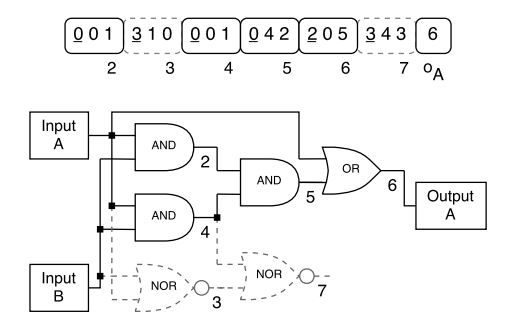
\includegraphics[width=0.5\linewidth]{pre_mutation}
 	\caption{Logički sklop prije mutacije izlaznog gena \cite{CGPbook}}
 \end{figure} 
 \begin{figure}[h]
	\centering
	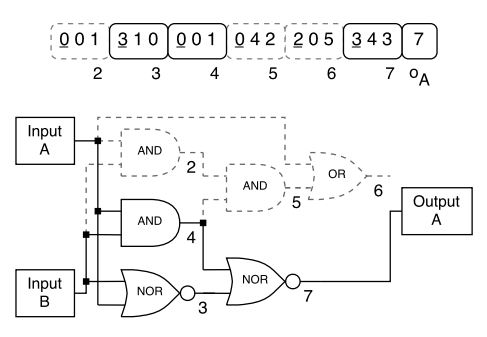
\includegraphics[width=0.5\linewidth]{post_mutation}
	\caption{Logički sklop nakon mutacije izlaznog gena iz 6 u 7 \cite{CGPbook}}
\end{figure}
\par
Mutacija nekodirajućeg gena na prvu ne pokazuje rezultate, ali je iznimno bitna. Pokazali smo kako izmjena gena fenotipa može bitno utjecati na sastav fenotipa tako da nekodirajući geni postanu kodirajući. Prema tome, svaki nekodirajući gen ima šansu postati kodirajući i sve izmjene nad njim mogu postati korisne ili štetne za rad programa. Iako nam učinak izmjene nije poznat u trenutku uspoređivanja, ovo je jedan od razloga zbog kojih u elitizmu i selekciji odabiremo djecu, a ne roditelje, ako se ispostavi da imaju jednaku dobrotu \cite{CGPbook}\cite{CGPpresentation}. 
\par
Jedan od oblika implementacije mutacije programa izmjena je nasumičnih gena dok se ne izmijeni određen postotak genotipa \cite{CGPbook}. Postotak određuje osoba koja radi implementaciju. Prilikom određivanja postotka važno je imati na umu da prevelika mutacija dovodi do destruktivnih posljedica za populaciju programa. 
\par
"Single mutation" naziv je za implementaciju mutacije gdje se izmjena gena provodi dok se ne izmjeni kodirajući gen \cite{CGPpresentation}. Ova implementacija cilja na promjenu fenotipa i ne postoji ograničenje na broj izmjena koje će se izvesti do ispunjenja uvjeta. 

\chapter{Implementacija}
\quad U ovom poglavlju obrađujemo implementacijske detalje sustava baziranog na CGP-u korištenog u radu i promjene učinjenje u verziji korištene igre.
\section{Osnovne informacije}
\quadČitava implementacija napravljena je u programskom jeziku Java (verzija 19.0.1). Sustav baziran na CGP-u napravljen je u obliku klase imena \textit{CGP} i ukomponiran je u paket igre. Sustav stvara i koristi dodatne dvije txt datoteke u kojima se drže rezultati treniranja (\textit{scores.txt}) i zadnja populacija programa s kojom je sustav radio (\textit{population.txt}). Programi se zapisuju u obliku niza brojeva po uzoru na zapis opisan u poglavlju 4 uz parametar l=$ n_{c} $. Modifikacije verzije igre napravljene su u postojećim klasama.
\par 
Sustav za treniranje programa koncipiran je poput podržanog učenja s brojem generacija kao uvjetom zaustavljanja. Program nakon kraja igre dobiva rezultat (eng. score) koji služi kao dio dobrote programa. Svaki program ima unaprijed zadan broj ponavljanja igranja igre. Ponavljanja su uvedena zbog elemenata nasumičnosti igre i njima se pokušava smanjiti utjecaj elemenata na ocjenu uspješnosti programa. Konačna ocjena uspješnosti programa bit će dana nakon zadnjeg ponavljanja i bit će srednja vrijednost svih dobivenih rezultata.
\par
\section{Programi}
\quad Implementacijska ideja kreće od koncepta programa. Koje podatke prenijeti programu? Kako bi program trebao signalizirati svoju odluku o smjeru pomicanja elementa?
\par
Radi olakšanja rada, programi su tijekom treniranja sadržani u objektima klase \textit{Individula}. Klasa \textit{Individual} sadržava: originalni zapis programa, program podijeljen u čvorove, rezultate dobivene igranjem igre, srednji rezultat igara, popis aktivnih čvorova, širinu mreže, dužinu mreže, broj čvorova, broj ulaza, broj izlaza i generacija nastanka. Svi podaci, osim rezultata, dani su pri samoj inicijalizaciji objekta.
\par 
Stanje ploče prenosi se programu u svakom koraku igre. S obzirom na to da ploča sadrži 16 polja, program ima 16 ulaza u mrežu. Stanje ploče prenosi se u obliku liste brojeva gdje se slijedno zapisuju polja ploče od gornje lijeve pozicije do donje desne. Brojevima od 0 do 12 zapisuje se sadržaj polja. 0 se koristi kao oznaka da je polje prazno, a ostali brojevi predstavljaju vrijednosti koje se mogu pojaviti u polju i možemo gledati na njih kao na eksponente na broj 2. U primjeru na slici 8.1 prva lista prikazuje početno stanje ploče. U početnom stanju vrijednost 2 pojavljuje se na dva mjesta; treći red i četvrti stupac, četvrti red i treći stupac.
 \begin{figure}[h]
	\centering
	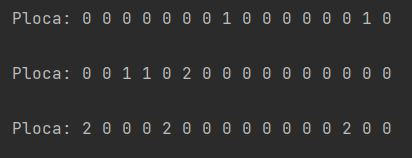
\includegraphics[width=0.6\linewidth]{imp_4}
	\caption{Stanje ploče tijekom tri poteza}
\end{figure}

\par
Završetkom obrade podataka u mreži, konačni rezultati dovode se na četiri izlaza. Svaki izlaz signalizira pokret u određenom smjeru (gore, desno, dolje, lijevo). Izlaz s najvećom vrijednošću predstavlja odluku programa.
\par
Stanje ploče nije bilo praćeno u igri te je uvedeno tijekom ovog rada u klasu \textit{Spavner}. Uvođenjem modifikacija u klasu, \textit{Spavner} pohranjuje i obnavlja stanje ploče nakon svakog poteza. Ustanovi li se da je ploča puna i da više nema mjesta za novi element, ploča se čisti, a sprema se lista nula koja signalizira da je igra završila. Završetkom igre programu se šalje rezultat partije. Nakon takvog kraja igre ploča se ponovo postavlja u početno stanje spremno za novu igru.
\
\par 
\section{Pokretanje treniranja}
\quad Sustav za treniranje programa može se pokrenuti na dva načina. Nakon pokretanja igre, pritiskom na tipku \textit{0} pokreće se metoda sa slike 8.2 koja briše zapis prošle generacije s kojom je sustav radio iz \textit{population.txt}, ako postoji; stvara se nova početna generacija i započinje treniranje.
\begin{figure}[h]
	\centering
	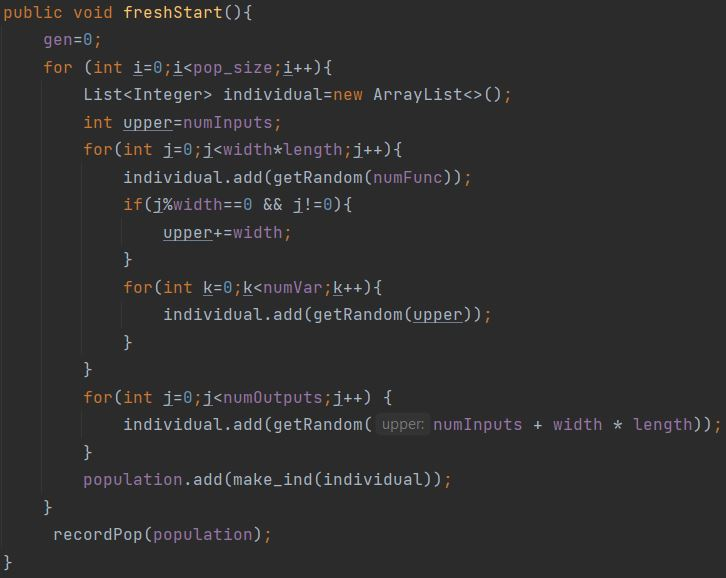
\includegraphics[width=0.6\linewidth]{fresh_start}
	\caption{Metoda inicijalizacije nove početne populacije aktivirana pritiskom na tipku \textit{0}}
\end{figure}
\par Pritiskom na tipku \textit{4} nastavljamo treniranje populacije zapisane u \textit{population.txt}. Populacija se zapisuje u \textit{population.txt} prilikom inicijalizacije sasvim nove populacije ili nakon generiranja nove generacije. Dodatni parametri koji se šalju u zapis osim programa su širina i duljina mreže te trenutna generacija. Slika 8.3 prikazuje metodu koja zapisuje populaciju.
\begin{figure}[h]
	\centering
	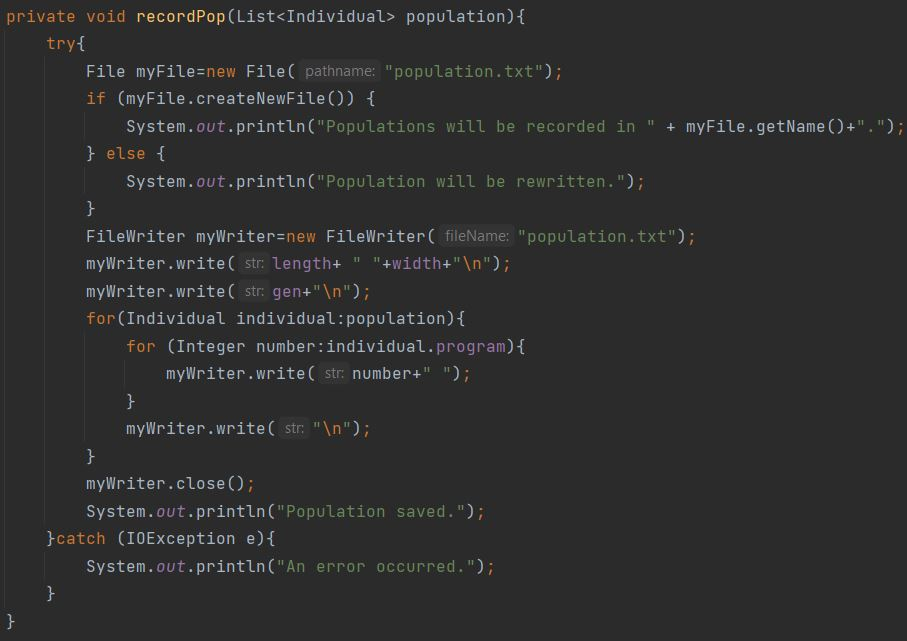
\includegraphics[width=0.6\linewidth]{recordPop}
	\caption{Metoda spremanja populacije u \textit{population.txt}}
\end{figure}\newline
\par
 Početni parametri programa i sustava (broj redova, broj stupaca, veličina populacije, broj ponavljanja) zadaju se u \textit{KeyInput} klasi kod inicijalizacije objekta klase CGP. Dodatni parametri poput generacijske granice, mogućih funkcija i broja mutacija mogu se podesiti unutar klase \textit{CGP}, s napomenom kako promjena mogućih funkcija zahtijeva više promjena implementacije i veći oprez.
\par
Zadnji korak u pokretanju treniranja je stvaranje dretve koja će provoditi treniranje. Ovime glavnu dretvu vraćamo održavanju igre i grafičkog sučelja te postižemo paralelan rad.
\section{Igranje igre}
\quad Dretva zadužena za treniranje kontinuirano dohvaća stanje ploče. Ako na ploči postoje elementi, stanje ploče se prosljeđuje metodi \textit{predict} (Slika 8.4) koja izvodi trenutni program na način koji je opisan u potpoglavlju 4.6. Metoda vraća broj izlaza s najvećom vrijednosti. Odluka o pomicanju elemenata donosi se na osnovu dobivenog broja. 
\par
Ako na ploči nema elemenata to znači kako je igra završila. Spremamo rezultate i pozivamo metodu \textit{keep\_count} (slika 8.5) koja prati koji program se izvodi, koliko puta se izveo i nalazimo li se na prijelazu u novu generaciju.
\begin{figure}[h]
	\centering
	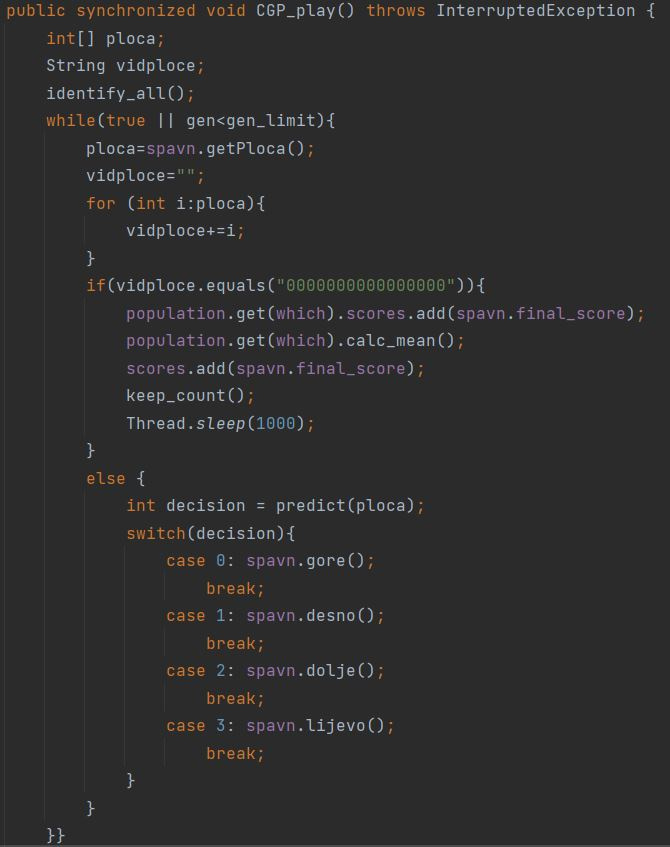
\includegraphics[width=0.6\linewidth]{cgpPlay}
	\caption{Metoda kontinuiranog provođenja igranja igre}
\end{figure}\newline
\begin{figure}[h]
	\centering
	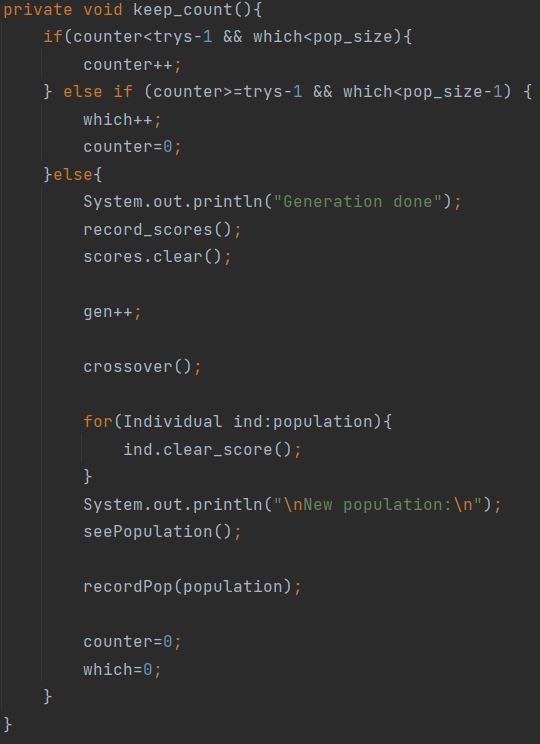
\includegraphics[width=0.6\linewidth]{keep_count}
	\caption{Metoda praćenja programa i generacija}
\end{figure}\newline
\section{Selekcija i križanje}
\quad Metoda \textit{keep\_count} prepoznaje kraj generacije, zapisuje vrijeme zapisa, parametre sustava, rezultate svakog programa i pokreće operaciju selekcije i križanja. Selekcija je implementirano kao turnir s nasumičnim izborom programa. Broj programa koje odabiremo je varijabilan, ali je uvijek višekratnik broja četiri. Razlog tome je taj da odabiremo dva para po dva programa. Programe u paru međusobno uspoređujemo. Programi koji su unutar para bili bolji križaju se, a gori će biti zamijenjeni djecom boljih. Bolji programi i programi koji nisu sudjelovali u turnirima prelaze u novu generaciju. Ovime se donekle ostvaruje elitizam jer najbolji programi na jedan ili na drugi način prelaze u sljedeću generaciju.
\par 
Implementirane su dvije metode križanja. Prva metoda se može smatrati destruktivnom i najmanje je korištena u testovima. Implementirana je za mreže sa širinom većom od jedan. Metoda stvara dvoje djece tako da svaki čvor djeteta ima 50\% šanse doći od jednog ili od drugog roditelja. Destruktivnost proizlazi iz činjenice da se na ovaj način genima jednog roditelja remete dijelovi genotipa drugog roditelja koji su ga činili uspješnim. (Slike 8.6 (a) i (b))
\begin{figure}[h]
	\centering
	\begin{subfigure}{0.4\textwidth}
		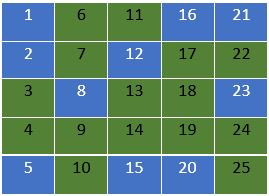
\includegraphics[width=0.9\linewidth]{my_cgp_cross_1} 
		\caption{Prvo dijete}
	\end{subfigure}
	\begin{subfigure}{0.4\textwidth}
		{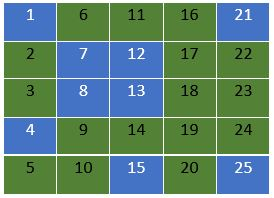
\includegraphics[width=0.9\linewidth]{my_cgp_cross_2}}
		\caption{Drugo dijete}
	\end{subfigure}
	\caption{Primjer rezultata prve metode križanja}
\end{figure}
\par
Druga metoda implementirana je za mreže širine 1 i zasnovana je na križanju s jednom točkom prijeloma. Kopije dva roditelja se prepolove u odabranom čvoru, a zatim se svaki dio spoji s dijelom drugog programa. 
\begin{figure}[h]
	\centering
	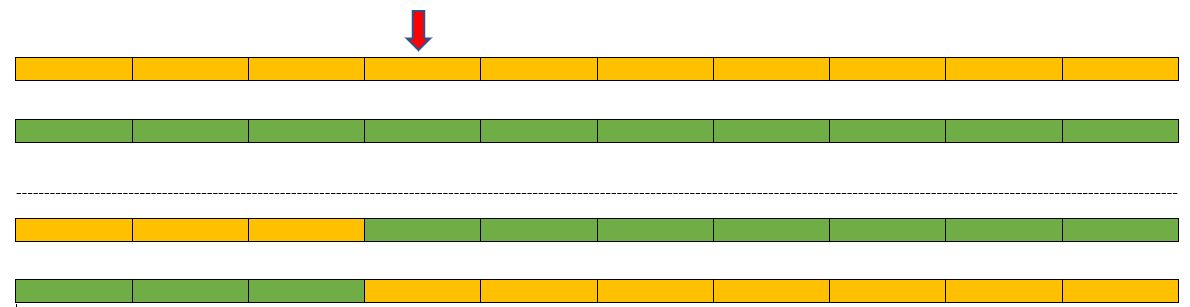
\includegraphics[width=0.6\linewidth]{crossover_point}
	\caption{Križanje s jednom točkom prijeloma}
\end{figure}

\section{Mutacija}
\quad Implementirane su dvije vrste mutacija, mutacija postotka i single mutacija, ali u testovima je korištena samo single mutacija kako bi se smanjila mogućnost potencijalno prevelike promjene fenotipa. Implementacija (Slika 8.8) dodatno omogućuje odabir broja uzastopnih single mutacija djeteta u svrhu proširenja područja testiranja. Single mutacija olakšana je činjenicom da objekti klase \textit{Individual} već sadrže popis aktivnih gena pa stvaramo listu gena za mutaciju dok ne odaberemo gen s popisa aktivnih gena. Jednom kad se aktivni gen odabere, prestajemo tražiti gene za mutaciju, a odabrane gene izmijenimo.
\par 
 Mutacijom završavamo naš proces stvaranja djece. Novonastala djeca pridružuju se već postojećoj populaciji dolaskom na mjesto programa koji su se iskazali slabijima u procesu selekcije. Time započinjemo novu generaciju, a podaci o novoj populaciji spremaju se u \textit{population.txt}
 
\begin{figure}[h]
	\centering
	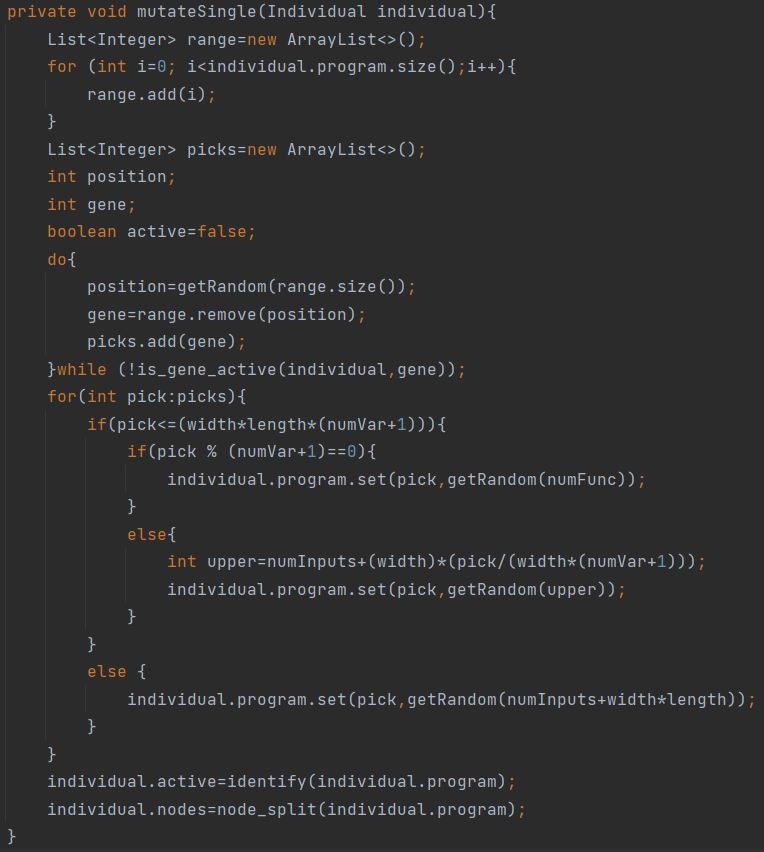
\includegraphics[width=0.6\linewidth]{my_cgp_mutation}
	\caption{Metoda Single mutacije}
\end{figure}

\newpage
\verb| |

\chapter{Rezultati}
\quad Testovi su izvođeni na već opisanoj verziji igre \textit{2048}. Verzija se ispostavila problematičnom jer je brzina izvođenja igre bitno ograničena implementacijom verzije. U svim testovima svi su programi imali tri pokušaja rješavanja igre. U slučaju veličine populacije četiri, prosječno vrijeme potrebno za prolazak svih programa generacije kroz igru bilo je petnaest minuta. U slučaju veličine populacije osam, prosječno vrijeme prolaska generacije kroz igru bilo je trideset minuta. U slučaju veličine populacije šesnaest, prosječno vrijeme prolaska generacije kroz igru bilo je šezdeset minuta. Povećanje potrebnog vremena je linearne zavisnosti i učinilo je treniranje predugim za ikakve prave rezultate. Rezultati koji su prikupljeni za različite arhitekture i parametre sustava ograničeni su na tridesetu generaciju kako bi se mogli međusobno usporediti. Ograničenje je takvo zbog toga što je to minimalna generacija do koje su došli svi testovi prije zaustavljanja daljnjeg treniranja. 
\par
Provedeno je pet testova s četiri različite arhitekture i s različitim parametrima sustava. Radi jednostavnosti zapisa ispod slika uvodimo kratice: c - broj stupaca, r - broj redova, p - veličina populacije, f - broj funkcija, m - broj mutacija po djetetu.
 \par
 Prvi test izveden je nad arhitekturom mreže sa širinom šesnaest i dubinom četiri uz veličinu populacije četiri, broj funkcija četiri (+,-,*,/) i jednom single mutacijom po djetetu. Selekcija se provodi nad četiri programa. Korišteno je križanje koje je prvo opisano u potpoglavlju 8.5. Test je osmišljen kao reprezentacija općenite i plitke mreže sa širinom većom od nula, a u ovom slučaju širina je jednaka broju ulaza. Trajanje testiranja bilo je 24 sata, unutar kojih je sustav prošao kroz sedamdeset i dvije generacije. Većina rezultata nalazila se u rasponu 70-150. Na slici 9.1 možemo vidjeti najbolje srednje vrijednosti rezultata od nulte do tridesete generacije. Iako oscilacije postoje, vidimo polagani rast najboljih rezultata do petnaeste generacije gdje započinje stagnacija i lagan pad. Na osnovu rezultata daljnjih generacija, srednje vrijednosti rezultata stagniraju ili se nalaze unutar istog raspona rezultata.
 \begin{figure}[h]
 	\centering
 	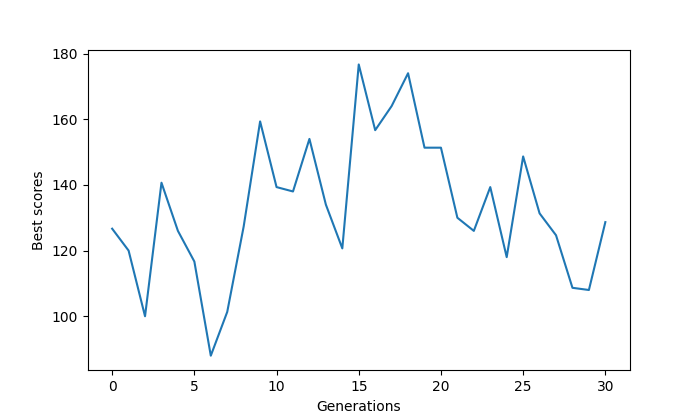
\includegraphics[width=0.9\linewidth]{graph_1}
 	\caption{Najbolje srednje vrijednosti rezultata programa za c=4, r=16, p=4, f=4, m=1}
 \end{figure}\newpage
\par
Drugi test izveden je nad arhitekturom mreže sa širinom jedan i dubinom sto uz veličinu populacije četiri, broj funkcija četiri (+,-,*,/) i jednom single mutacijom po djetetu. Selekcija je provedena nad četiri programa. Korišteno je križanje s jednom točkom prijeloma. Test je osmišljen kao reprezentacija jednostavnog slučaja mreže širine jedan gdje je naglasak na vezama između čvorova u dubini. Ideja je bila koristiti ovaj slučaj kao bazu za uspoređivanje s drugim arhitekturama i parametrima sustava. Trajanje testiranja bilo je 22 sata, unutar koji je sustav prošao kroz pedeset i tri generacije. Većina rezultata nalazila se u rasponu 90-150. Na slici 9.2 možemo vidjeti najbolje srednje vrijednosti rezultata od nulte do tridesete generacije. Primjećuje se porast najbolje srednje vrijednosti do dvadeset i treće generacije nakon čega slijedi nagli pad uspješnosti i povratak u stanje prije pada. Rezultati daljnjih generacija ukazuju na umjereno poboljšanje, ali gornja granica raspona većine rezultata ne pomiče se previše.
\par 
Treći test je gotovo po svim parametrima jednak prošlom. Jedina razlika je veličina populacije. U ovom testu veličina populacije je 8. Cilj ovog testa bio je vidjeti razliku u uspješnosti kroz generacije ako povećamo veličinu populacije. Trajanje testiranja bilo je 20 sati, unutar kojih je sustav prošao kroz trideset i dvije generacije. Većina rezultata nalazi se u rasponu od 80-150. Počinjemo uviđati iste raspone rezultata kroz testove i sumnja se kako je ovo početni raspon rezultata većine inicijaliziranih populacija. Slika 9.3 prikazuje najveće srednje vrijednosti rezultata od nulte do tridesete generacije. Stabilan porast rezultata u ovom testu kasni za onim u prošlom testu. Minimalna i maksimalna vrijednost rezultata je veća od prošlog testa, iako je razlika možda zanemariva.

 \begin{figure}[h]
	\centering
	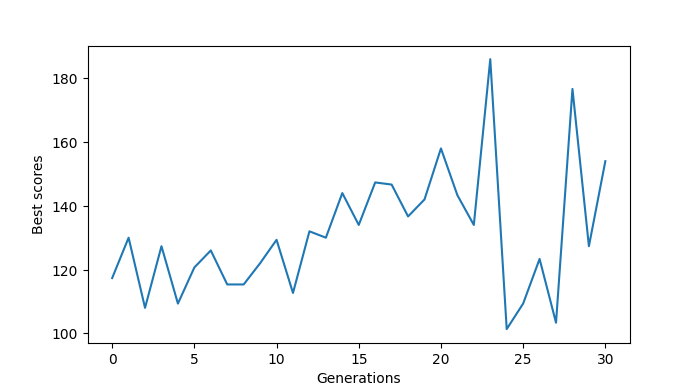
\includegraphics[width=0.9\linewidth]{graph_2}
	\caption{Najbolje srednje vrijednosti rezultata programa za c=100, r=1, p=4, f=4, m=1}
\end{figure}

 \begin{figure}[h]
	\centering
	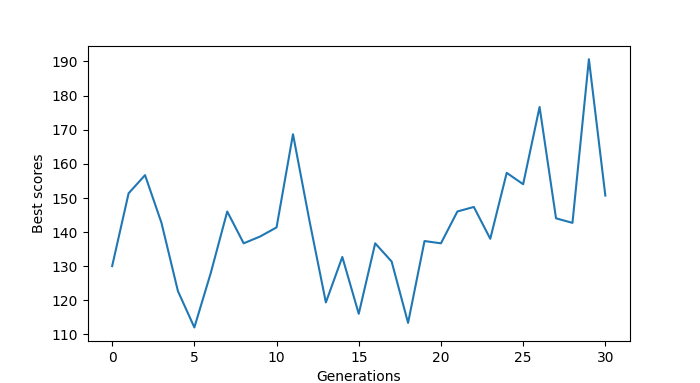
\includegraphics[width=0.9\linewidth]{graph_3}
	\caption{Najbolje srednje vrijednosti rezultata programa za c=100, r=1, p=8, f=4, m=1}
\end{figure}

\par
U četvrtom testu dubina je povećana na dvjesto i uvedene su još dvije funkcije (min i max). Testom se pokušao vidjeti utjecaj produbljavanja mreže i dodavanja dodatnih mogućih funkcija. Trajanje testiranja bilo je 20 sati, unutar kojih je sustav prošao kroz trideset i pet generacija. U početnim generacijama većina rezultata nalazi se u rasponu 100-150, ali u kasnijim generacijama raspon pada na 90-120. Slika 9.4 prikazuje najveće srednje vrijednosti rezultata od nulte do tridesete generacije. Iznos najveće srednje vrijednosti rezultata u generaciji je nestabilan te na odsječku od trideset generacija ne možemo zaključiti previše. Prosjek rezultata po generacijama pokazuje stabilizaciju rezultata, ali i njihov pad. 
 \begin{figure}[h]
	\centering
	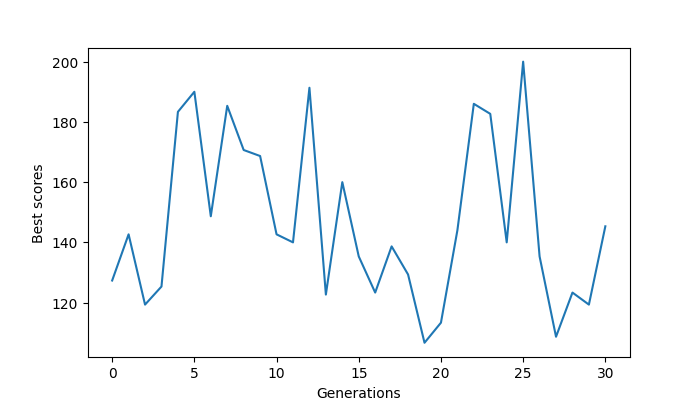
\includegraphics[width=0.9\linewidth]{graph_4}
	\caption{Najbolje srednje vrijednosti rezultata programa za c=200, r=1, p=8, f=6, m=1}
\end{figure}

\par
Peti test nadograđuje četvrti tako da smo mrežu produbili s dodatnih sto čvorova, veličinu populacije postavili na šesnaest, selekcija je provedena nad osam programa i broj single mutacija po djetetu povećali na dva. Cilj testa bio je vidjeti kako će povećanje kompleksnosti i promjenjivosti populacije utjecati na rezultate. Trajanje testiranja bilo je 43 sata, unutar kojih je sustav prošao kroz četrdeset i jednu generaciju. Većina rezultata nalazi se u rasponu od 90-150. Slika 9.5 prikazuje najveće srednje vrijednosti rezultata od nulte do tridesete generacije. Najveća srednja vrijednost rezultata generacije u ovom testu postiže najveći iznos u usporedbi s ostalim testovima. Na žalost ovaj test jedini pokazuje jasan pad najveće srednje vrijednosti rezultata i izrazito je nestabilan s naglim usponima i padovima.  
 \begin{figure}[t]
	\centering
	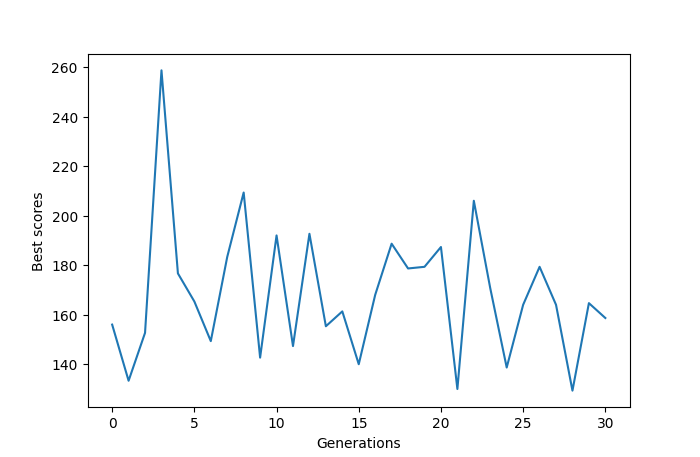
\includegraphics[width=0.9\linewidth]{graph_5}
	\caption{Najbolje srednje vrijednosti rezultata programa za c=300, r=1, p=16, f=6, m=2}
\end{figure}
\par 
Pregledom rezultata testova možemo pretpostaviti nekoliko učinaka koje parametri mogu imati na uspješnost programa. Veća kompleksnost može dovesti do većeg uspjeha programa, ali dovodi i do veće nestabilnosti. Prevelika razina mutacije utječe destruktivno na generacije programa. Povećavanjem populacije, bez povećanja selekcije, može dovesti do odgađanja promjene u populaciji. Sve ove pretpostavke nisu dokazane već su postavljene na osnovu dobivenih rezultata i trebaju se tretirati kao moguće hipoteze za budući rad.
\newpage
\verb| |

\chapter{Zaključak}
\quad Uloga genetskih algoritama u strojnom učenju neosporiva je i značajna u današnjem svijetu. Nevjerojatna je učinkovitost  metode pogreške i pokušaja koja kroz generacije programa stvara najbolja rješenja za različite probleme i okoline u kratkom roku. Fascinantnost ovakvog oblika učenja i razvoja programa uvjetovala je stvaranje ovog rada. 
\par 
Tijekom ovog rada, pomoću Kartezijevog genetskog programiranja, razvijeni su agenti čiji je cilj igranje igre \textit{2048}. Objašnjena su pravila i funkcioniranja verzija igara, objašnjeni su ključni elementi i operacije genetskog programiranja i Kartezijevog genetskog programiranja, izložena je i objašnjena implementacija rada, izvedeni su i prikazani rezultati testova implementacije.
\par 
Na žalost, verzija igre učinila se previše problematičnom za skupljanje veće količine podataka i provođenje više testova. Određeni napreci, nazadovanja i utjecaji parametara mogu se vidjeti, ali za pravi učinak morali bi moći provesti razvoj kroz podosta više generacija nego što je provedeno u ovom radu. 
\par
Implementacija otvara mogućnosti za daljnji rad i istraživanje. Potencijalne modifikacije bile bi olakšavanje unosa i korištenja određenih parametara sustava uz moguće grafičko sučelje koje bi zamijenilo potrebu za unošenjem parametara direktno u programski kod implementacije. Kombinacije različitih parametara gotovo su neograničene i ostavljaju puno prostora za daljnja testiranja. Najveći napredak može se postići dodatnim radom na korištenoj verziji igre, upotrebom druge verzije ili razvojem vlastite kojom bi se ubrzalo vrijeme treniranja i razvoja programa. 

\bibliography{literatura}
\bibliographystyle{fer}

\begin{sazetak}
Cilj ovog rada je stvoriti agenta ili populaciju agenata koji će naučiti igrati igru 2048. Učenje se provodi korištenjem Kartezijevog genetskog programiranja. U sklopu ovog rada obrađuju se koncepti genetskog programiranja, Kartezijevog genetskog programiranja, razvoja agenata kroz generacije, izlaže se implementacija rada u programskom jeziku Java, prikazuju se rezultati testiranja implementacije, diskutiraju se dobiveni rezultati i predlažu se potencijalna poboljšanja.

\kljucnerijeci{Igra 2048, genetski algoritam, genetsko programiranje, Kartezijevo genetsko programiranje}
\end{sazetak}

% TODO: Navedite naslov na engleskom jeziku.
\engtitle{Playing the 2048 game using Cartesian genetic programming}
\begin{abstract}
The goal of this thesis is to create an agent or a population of agents that will learn to play the game 2048. The learning is performed using Cartesian genetic programming. As part of this work, the concepts of genetic programming, Cartesian genetic programming and the development of agents through generations are discussed, the implementation of the work in Java programming language and the results of implementation testing are presented, the obtained results are discussed and potential improvements are proposed.

\keywords{Game 2048, genetic algorithm, genetic programming, Cartesian genetic programming}
\end{abstract}

\end{document}
